\subsection{Stagnation flow}
% ----------
\begin{figure}
\begin{center}
\begin{tabular}{ccc}
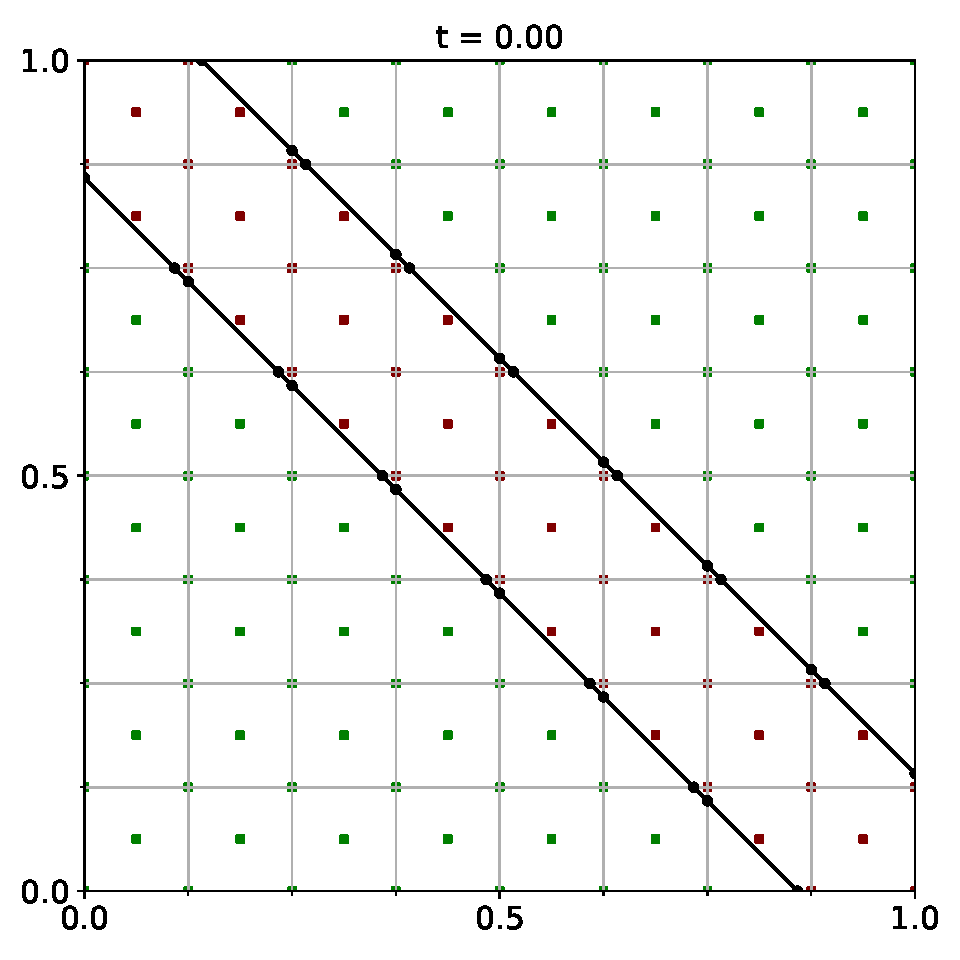
\includegraphics[width=0.3\textwidth]{stagnation_intf_0} &
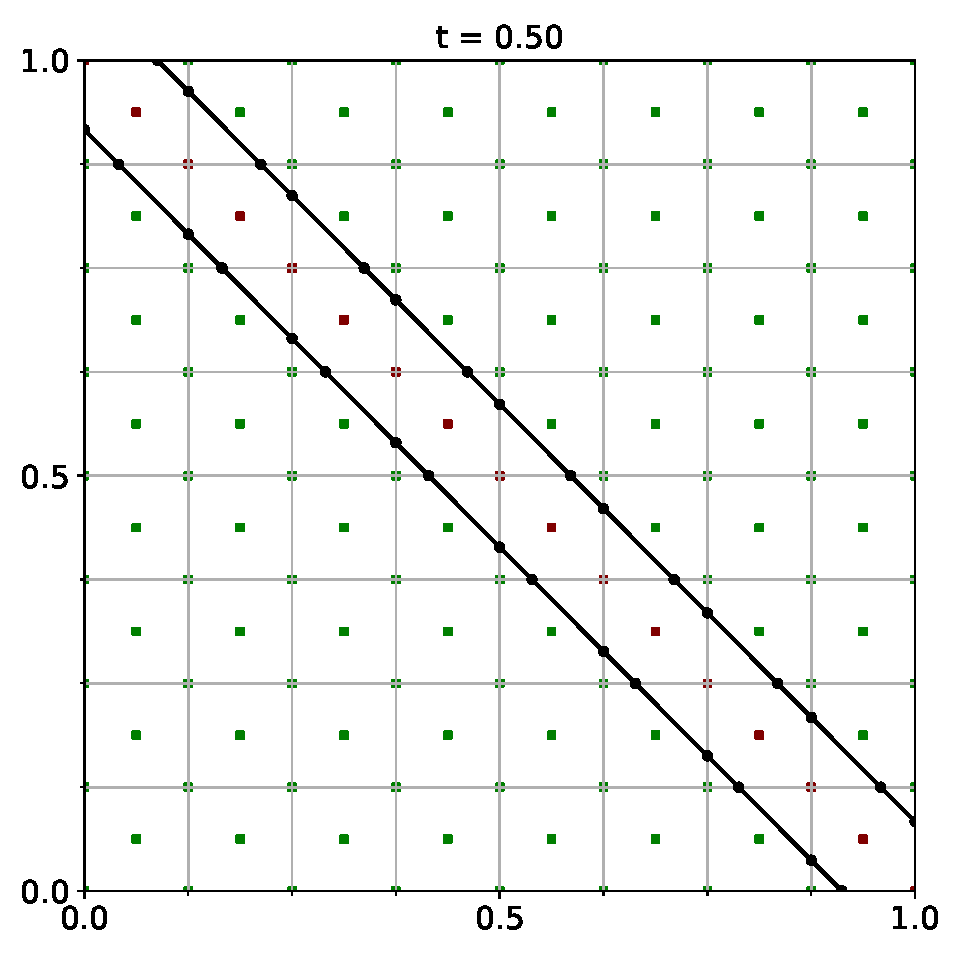
\includegraphics[width=0.3\textwidth]{stagnation_intf_32} &
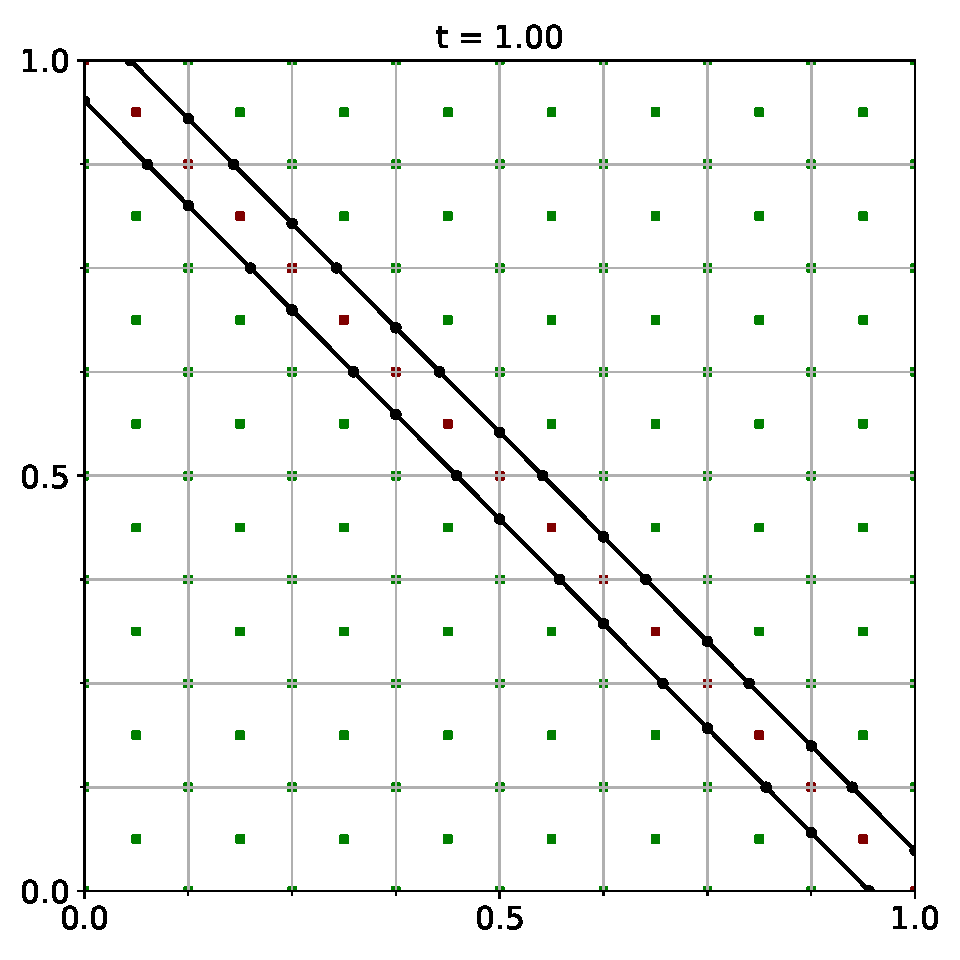
\includegraphics[width=0.3\textwidth]{stagnation_intf_64}
\\
(a) & (b) & (c)
\end{tabular}
\end{center}
\caption{Stagnation flow: interface lines and Color Vertex (reference phase is denoted by brown squares) at times $t = 0, 0.5, 1$.}
\label{Fig_stagna_intfs}
\end{figure}
% ----------

In this test two parallel linear interfaces oriented at $45$ degrees are placed inside the unit square domain. The initial thickness of the film is $D = 0.2$ (see Fig.~\ref{Fig_stagna_intfs}a). A stagnation flow $(u, v) = (0.5 - y, 0.5 - x)$ with a stagnation point at $(0.5, 0.5)$ is applied, so that the reference phase is drained out from the computational domain along a diagonal direction and the thickness of the film decreases. Eventually, a sub-cell film is formed inside the domain.
We consider this test only to show the capability of the EBIT method to preserve a sub-cell structure, therefore we use a rather coarse mesh with resolution $N_x \times N_x = 8 \times 8$ and a constant timestep $\Delta t = 1/64$ so that $CFL = u_{max} \Delta t / \Delta = 0.0625$.

The interface lines and the Color Vertex distribution at several times are shown in Fig.~\ref{Fig_stagna_intfs}. Initially, the film is thick enough so that there is no sub-cell structure (Fig.~\ref{Fig_stagna_intfs}a). As the drainage goes on, the film becomes thinner than the diagonal of the cell (Fig.~\ref{Fig_stagna_intfs}b) and it is correctly preserved by the EBIT method even at later times (Fig.~\ref{Fig_stagna_intfs}c).

\subsection{Translation with uniform velocity}

In this test a circular interface of radius $R=0.15$ and center at $(0.25, 0.75)$ is placed inside the unit square domain. The domain is meshed with $N_x \times N_x$ square cells of size $\Delta =1/N_x$, where $N_x = 32, 64, 128, 256, 512$. A uniform and constant velocity field $(u, v)$ with $u = -v$ is applied, so that the interface is advected along a diagonal direction. At halftime $t = 0.5\,T$ the center reaches the position $(0.75, 0.25)$, 
the velocity field is then reversed and the circular interface should return to its initial position at $t = T = 1$ with no distortion.

We use this case to test the new EBIT method, where the unaligned markers are computed by a circle fit. The accuracy and mass conservation of the method are measured by the area, shape, and symmetric difference errors. The area error $E_{area}$ is defined as the absolute value of the relative difference between the area occupied by the reference phase at the initial time $t=0$ and that at $t=T$
% ----------
\begin{equation}
E_{area} = \frac{|A(T) - A(0)|}{A(0)}
\label{Eq_error_surface}
\end{equation}
% ----------
The shape error, in a $L^\infty$ norm, is defined as the maximum distance between any marker $\boldsymbol{x}_i$ on the interface and the corresponding closest point on the analytical solution
% ----------
\begin{equation}
E_{shape} = \max\limits_i |dist (\boldsymbol{x}_i)|, \quad
dist (\boldsymbol{x}_i) = \sqrt{(x_i - x_c)^2 + (y_i - y_c)^2} - R
\label{Eq_error_shape}
\end{equation}
% ----------
where $(x_c, y_c)$ are the coordinates of the circle center and $R$ its radius. 
For all kinematic tests discussed in the following sections, the shape error is evaluated at the end of the advection.

For two domains, $A$ and $B$, the symmetric difference $A \bigtriangleup B$ is defined as follows
% ----------
\begin{equation}
A \bigtriangleup B = (A \cup B) \,\backslash\, (A \cap B)
\label{Eq_sym_diff}
\end{equation}
% ----------

In our test, the interface reconstructions at the beginning and at the end of the simulation are set to be $A$ and $B$, respectively. We use the area of symmetric difference
% ----------
\begin{equation}
E_{sym} = |A \bigtriangleup B| = |A| + |B| - 2 |A \cap B|
\label{Eq_sym_diff_error}
\end{equation}
% ----------
to measure the accuracy of an interface advection method.

To initialize the markers on the grid lines we first compute the signed distance \eqref{Eq_error_shape} on the cell vertices, then we use a root-finding routine, when the sign of the distance is opposite on the two endpoints of a cell side, to calculate the position of a marker. Hence, there is a small numerical error in the initial data, that accumulates as the interface is translated. However, because of the circle fit in the EBIT method this error remains rather limited during the translation.
We employ a relatively small $CFL$ number $CFL = (u\,\Delta t)/\Delta = 0.125$. The interface lines at halftime and at the end of the simulation are shown in Fig.~\ref{Fig_translation_intf} for different mesh resolutions. 

% ----------
\begin{figure}
\begin{center}
\begin{tabular}{cc}
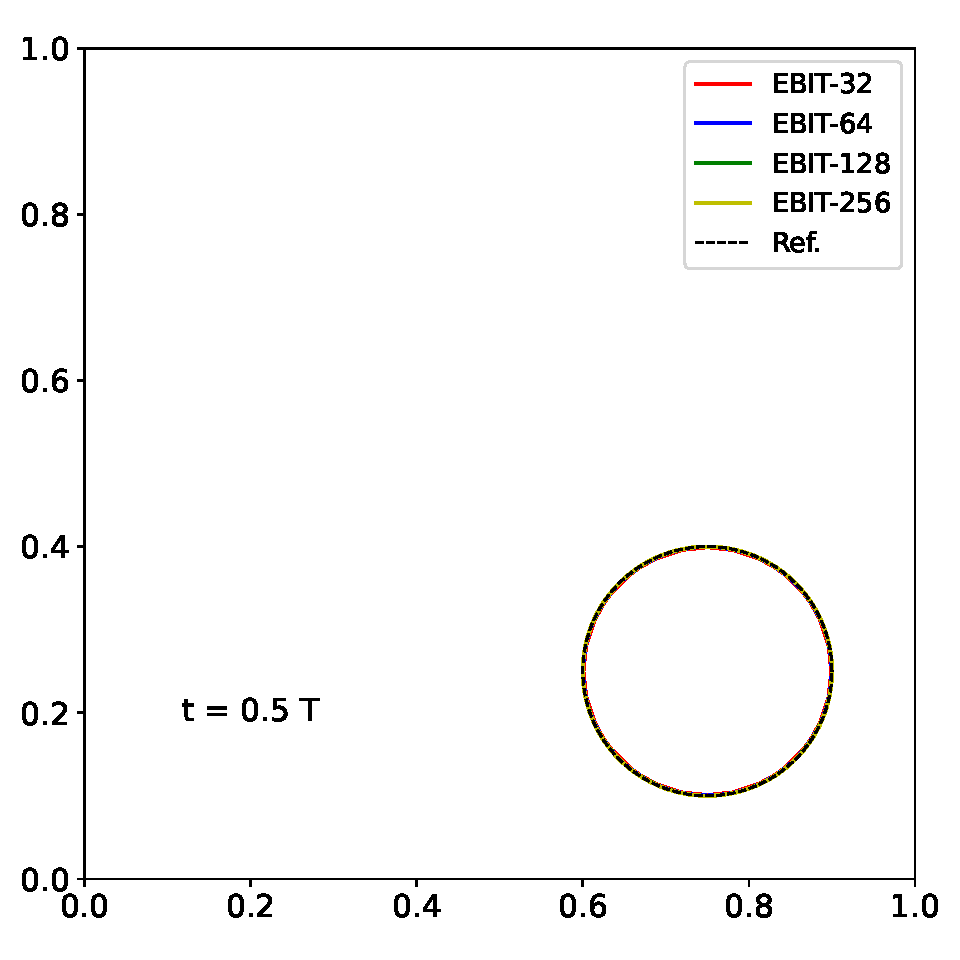
\includegraphics[width=0.45\textwidth]{circle_intf_1} &
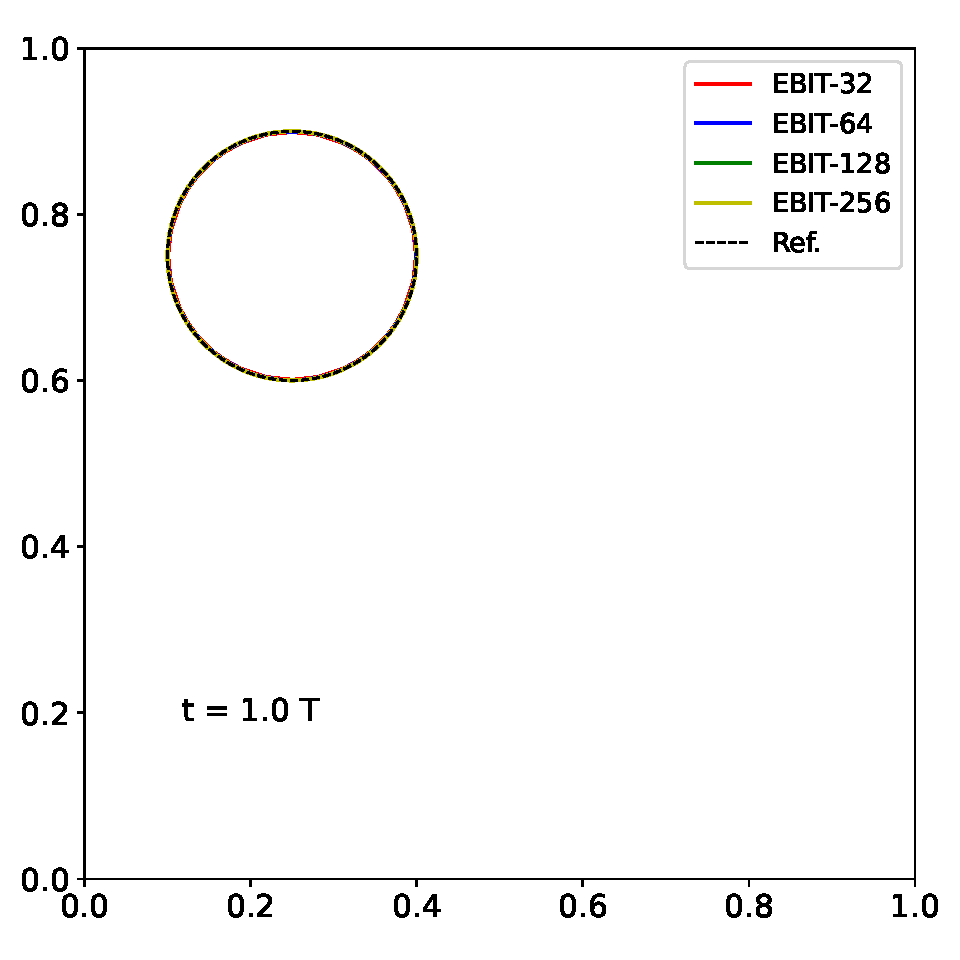
\includegraphics[width=0.45\textwidth]{circle_intf_2}\\
(a) & (b) 
\end{tabular}
\end{center}
\caption{Translation test with the new EBIT method at different resolutions: (a) interface lines at halftime; (b) interface lines at the end of the simulation.}
\label{Fig_translation_intf}
\end{figure}
% ----------
\begin{figure}
\begin{center}
\begin{tabular}{cc}
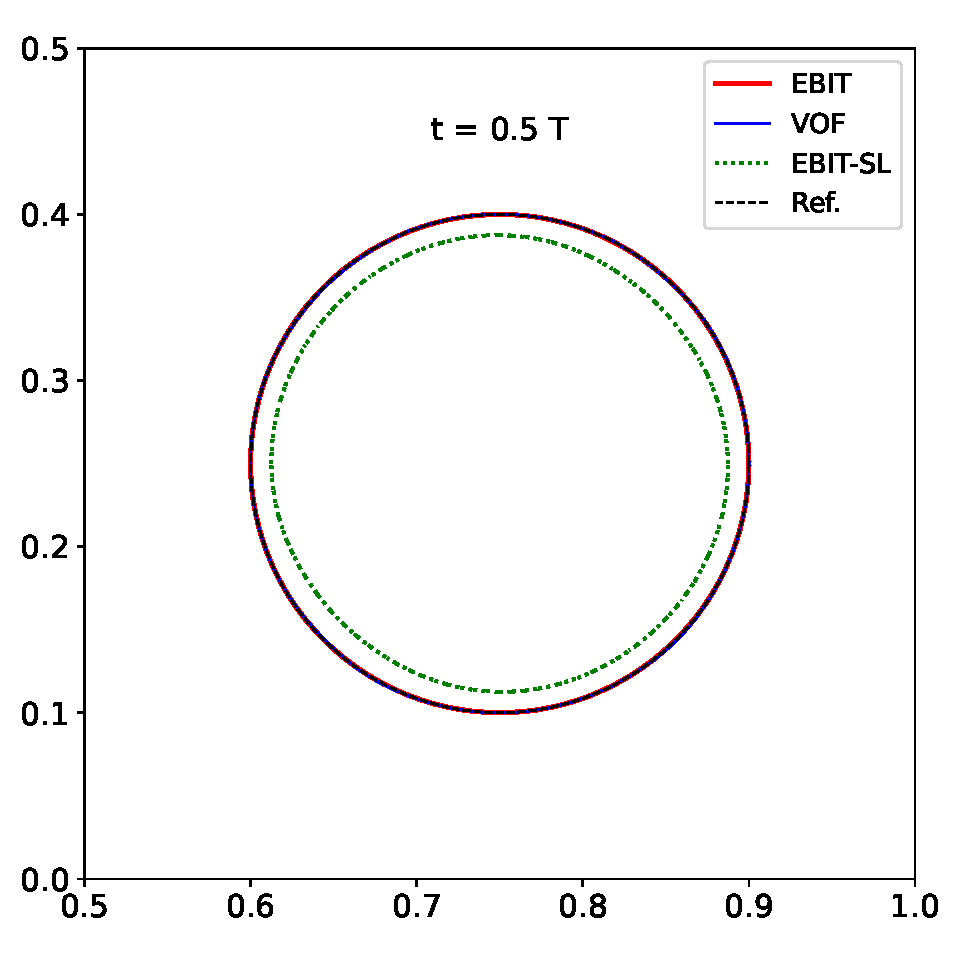
\includegraphics[width=0.45\textwidth]{circle_intf_vof_1} &
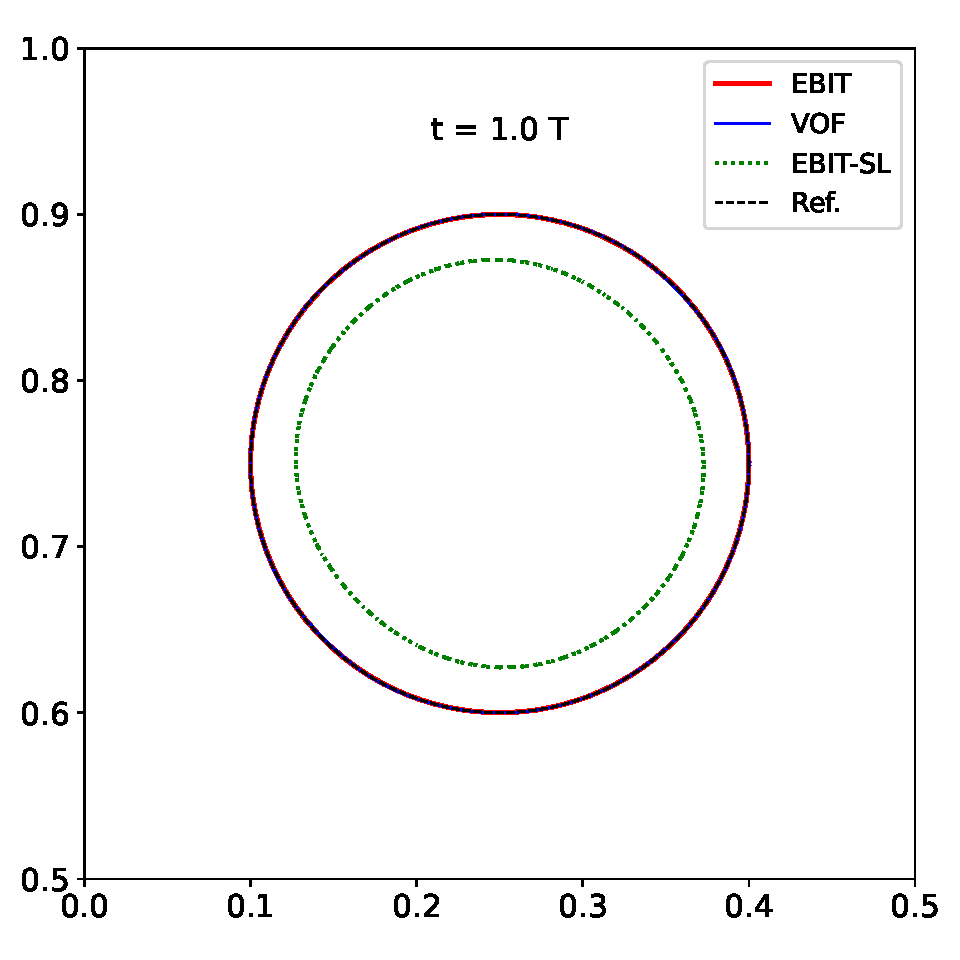
\includegraphics[width=0.45\textwidth]{circle_intf_vof_2}\\
(a) & (b) 
\end{tabular}
\end{center}
\caption{Translation test with different methods at resolution $N_x=128$: (a) interface lines at halftime; (b) interface lines at the end of the simulation.}
\label{Fig_translation_intf_cmp}
\end{figure}
% ----------
\begin{figure}
\begin{center}
\begin{tabular}{ccc}
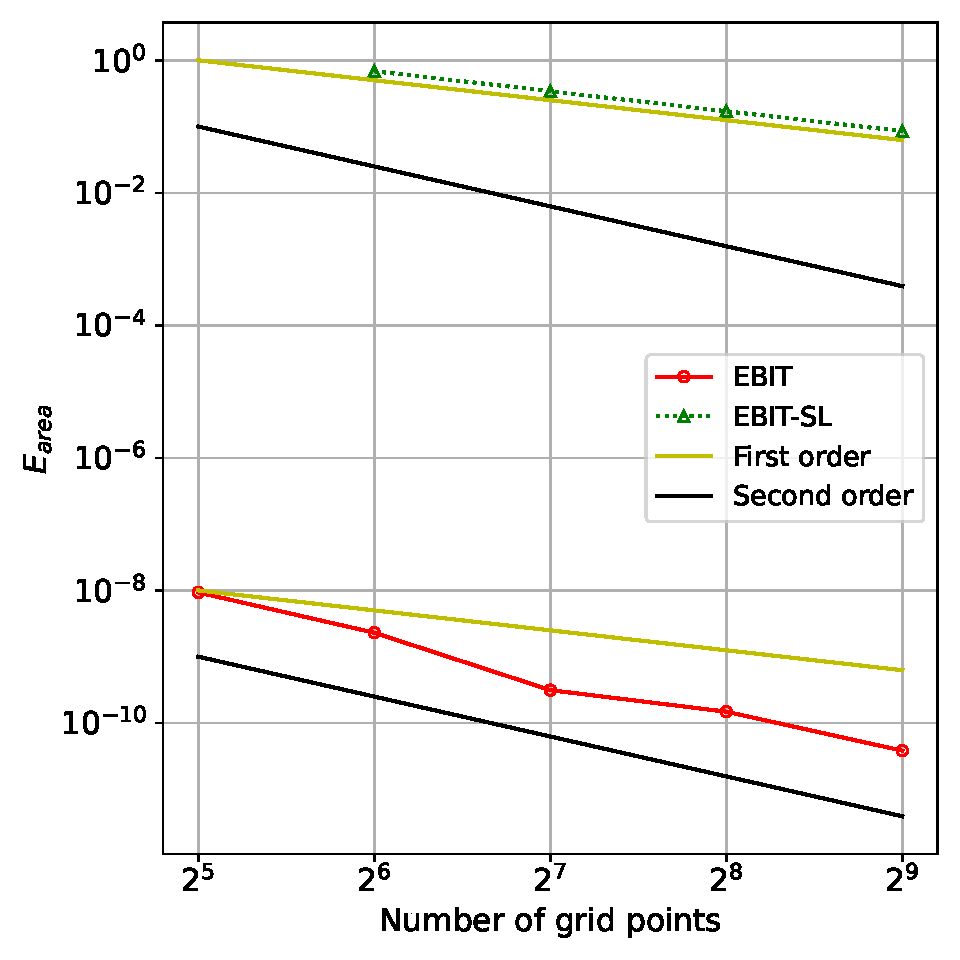
\includegraphics[width=0.33\textwidth]{circle_err_area} &
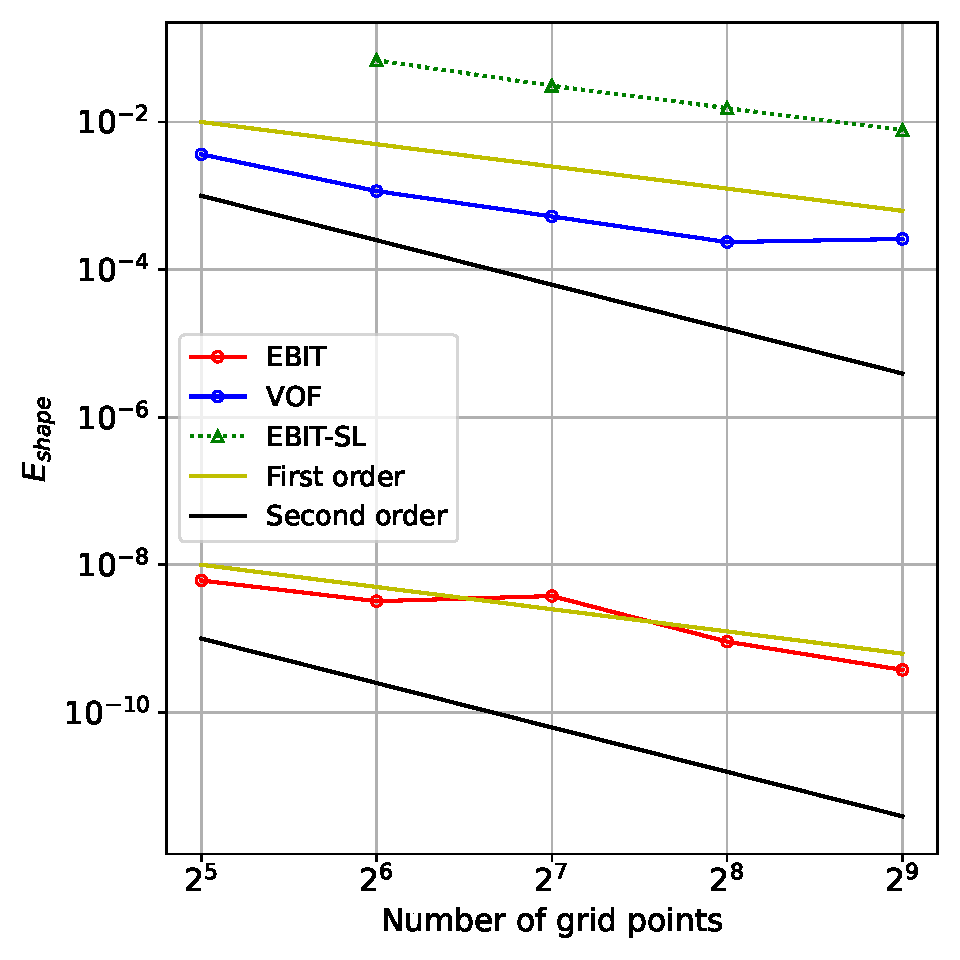
\includegraphics[width=0.33\textwidth]{circle_err_shape} &
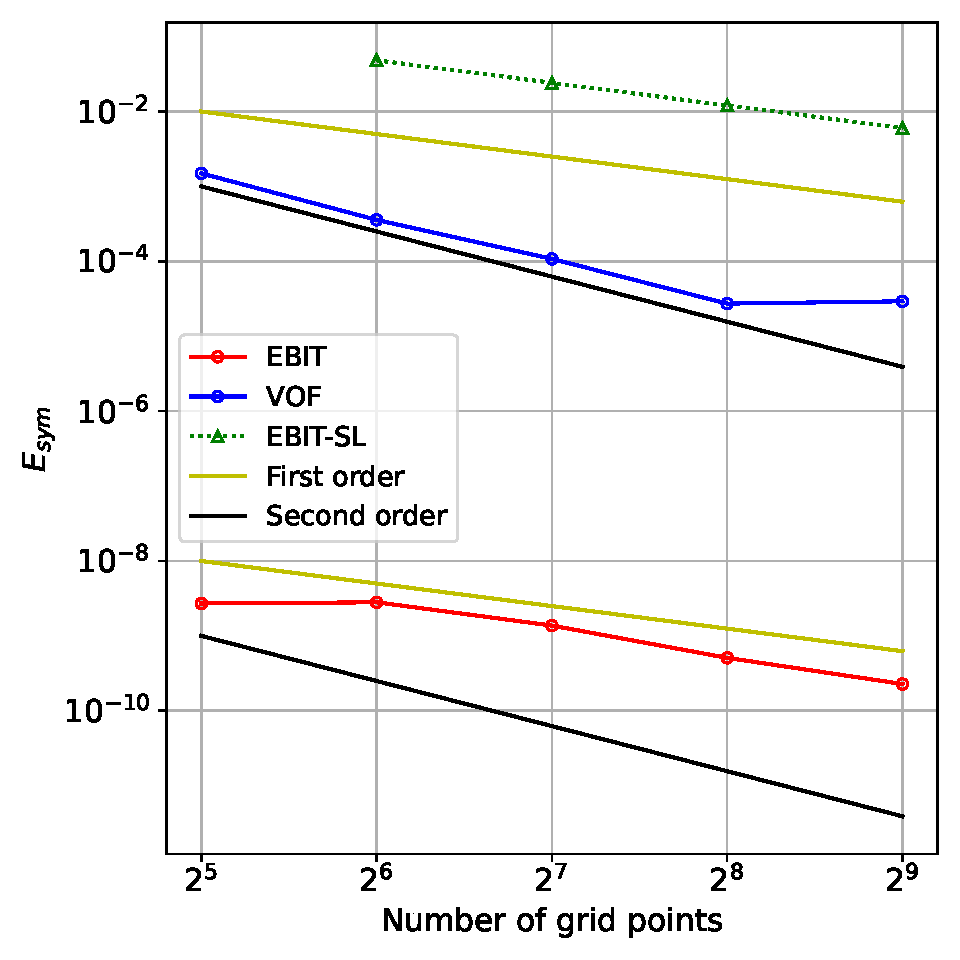
\includegraphics[width=0.33\textwidth]{circle_err_sym}\\
(a) & (b) & (c)
\end{tabular}
\end{center}
\caption{Errors in the translation test for different methods as a function of grid resolution: (a) area error $E_{area}$; (b) shape error $E_{shape}$; (c) symmetric difference error $E_{sym}$.}
\label{Fig_translation_error}
\end{figure}
% ----------

The interface lines are also calculated with different reconstruction and advection methods for a medium mesh resolution, $N_x = 128$, and are shown in Fig.~\ref{Fig_translation_intf_cmp}. Both the new EBIT method and the PLIC-VOF method maintain rather well the circular shape of the interface during the translation. On the other hand, the first version of the EBIT method, that considers a straight line approximation (SL) for the calculation of the position of unaligned markers, loses mass continuously during the simulation.

The area errors $E_{area}$ and the shape errors $E_{shape}$ are listed in Table~\ref{Tab_translation_error} and are shown in Fig.~\ref{Fig_translation_error} for the different methods. 
For the new EBIT method we observe a second-order convergence rate for the area error and approximately a first-order convergence rate for both the shape error and symmetric difference error, as shown in Fig.~\ref{Fig_translation_error}. For the first version of the EBIT method (SL), both the area, shape and symmetric difference errors are much larger. Furthermore, this method loses all the reference phase at the lowest grid resolution, $N_x = 32$ (this fact is denoted by ``NA'' in Table~\ref{Tab_translation_error}). 

% ----------
\begin{table}[hbt!]
\footnotesize
\caption{Mesh convergence study for the translation test.}
\centering
\begin{tabular}{cc|ccccc}
\hline 
 &$N_x$ &32 & 64 & 128 & 256 & 512\\ 
\hline 
EBIT&$E_{area}$ & $9.32\times 10^{-9}$ & $2.30\times 10^{-9}$ & $3.13\times 10^{-10}$ & $1.48\times 10^{-10}$ & $3.82\times 10^{-11}$\\ 
&$E_{shape}$ & $6.13\times 10^{-9}$ & $3.21\times 10^{-9}$ & $3.77 \times 10^{-9}$ & $9.08 \times 10^{-10}$ & $3.76\times 10^{-10}$\\
&$E_{sym}$ & $2.75\times 10^{-9}$ & $2.81\times 10^{-9}$ & $1.37 \times 10^{-9}$ & $5.09 \times 10^{-10}$ & $2.28\times 10^{-10}$\\
\hline 
VOF&$E_{shape}$ & $3.88\times 10^{-3}$ & $1.06\times 10^{-3}$ & $4.72 \times 10^{-4}$ & $2.59 \times 10^{-4}$ & $2.68\times 10^{-4}$\\
&$E_{sym}$ & $1.49\times 10^{-3}$ & $3.57\times 10^{-4}$ & $1.08 \times 10^{-4}$ & $2.73 \times 10^{-5}$ & $2.93\times 10^{-5}$\\
\hline 
EBIT-SL&$E_{area}$ & NA & $6.83\times 10^{-1}$ & $3.41\times 10^{-1}$ & $1.70\times 10^{-1}$ & $8.52\times 10^{-2}$\\ 
&$E_{shape}$ & NA & $6.86\times 10^{-2}$ & $3.10 \times 10^{-2}$ & $1.54 \times 10^{-2}$ & $7.78\times 10^{-3}$\\
&$E_{sym}$ & NA & $4.82\times 10^{-2}$ & $2.41 \times 10^{-2}$ & $1.20 \times 10^{-2}$ & $6.02\times 10^{-3}$\\
\hline 
\end{tabular}
\label{Tab_translation_error}
\normalsize
\end{table}
% ----------

For the PLIC-VOF method, the mass conservation is accurate to machine error and it is not shown in the figure, while the shape error is evaluated with the two endpoints of the PLIC-VOF reconstruction in each cut cell. For this error we observe in Fig.~\ref{Fig_translation_error} a first-order convergence rate. 
But for the symmetric difference error, we observe a second-order convergence rate. The lower order of convergence rate of the shape error may due to the discontinuous feature of the PLIC-VOF reconstruction on the cell edge and to the maximum norm we used for the evaluation of shape error.
Due to the fact that in the new EBIT method we are fitting a circle with a circle, the shape and symmetric difference errors obtained with the PLIC-VOF method are larger than those of the new EBIT method.

% ----------
\begin{table}[hbt!]
\caption{Performance in weak scaling on IRENE.}
\centering
\begin{tabular}{ccccc}
\hline 
 Number of cells & $N_c$ & $T_s$ ($10^{-3}$ s/step) & $S$/Ideal  & $E$ \\ 
\hline 
$128^2$ & $4$ & $2.16$ & $1 / 1$ & $1$ \\ 
$256^2$ & $16$ & $2.62$ & $3.3 / 4$ & $0.82$ \\ 
$512^2$ & $64$ & $2.80$ & $12.3 / 16$ & $0.77$ \\ 
$1024^2$ & $256$ & $3.26$ & $42.4 / 64$ & $0.66$ \\ 
$2048^2$ & $1024$ & $3.69$ & $149.7 / 256$ & $0.58$ \\ 
\hline 
\end{tabular}
\label{Tab_weak_scaling}
\end{table}
% ----------

We also use this simple case to test the scalability of the EBIT method. The simulations for the scalability test were run on ROME partition of the IRENE supercomputer. This partition contains 2286 nodes and each node contains 128 CPU cores. Only one thread is used for each CPU core, and each thread is mapped to an MPI process. 
For a Cartesian mesh, Basilisk employs a common domain decomposition strategy to subdivide the computational domain and distributes one subdomain to each MPI process. Since the markers are bound to a cell, as the interface moves across different subdomains, the markers are distributed to different processes automatically by the build-in subroutines of Basilisk.

For most of the 2D simulations, it is more reasonable to use a large number of cores when a very high resolution is needed. Hence we are more interested in the ``weak scaling'' performance of the EBIT method, where we vary the number of CPU cores and keep the number of cells distributed to each core fixed. A subdomain grid of $64 \times 64$ is used for test, and a minor difference of performance is observed when we further increase the resolution of the subdomain. The scalability is measured by the speedup $S(N_c)$ and efficiency $E(N_c)$:
% ----------
\begin{equation}
S(N_c) = \frac{N_c T_s (N_{c,ref})}{N_{c, ref} T_s (N_c)}, \quad E(N_c) = \frac{N_{c,ref} }{N_c} S (N_c)
\label{Eq_speedup}
\end{equation}
% ----------
where $N_c$ is the number of cores and $T_s$ the wall time per advection step. The number of cores used for reference ($N_{c, ref}$) is $4$. Table~\ref{Tab_weak_scaling} shows the overall performance of the EBIT method in weak scaling for five different runs.
For the ideal case without the overhead of communications and synchronizations among processes, the wall time should remain constant when the number of cores is increased. But due to the overheads in a real simulation, the wall time slightly increases as we increase the number of cores, as shown in Table~\ref{Tab_weak_scaling}. Consequently, the overheads incur a degradation of the speedup and efficiency and will eventually affect the overall scalability. The code is 149.7 times faster with 1024 cores, but the efficiency decreases to only $58\%$. Since this is our very first parallel study of the EBIT method, further optimization of the communications and synchronizations can still be performed to enhance its scalability.

\subsection{Single vortex}

The single vortex test was designed to test the ability of an interface tracking method to follow the evolution in time of an interface that is highly stretched and deformed \cite{Rider_1998_141}. A circular interface of radius $R=0.15$ and center at $(0.5, 0.75)$ is placed inside the unit square domain. 
A divergence-free velocity field $(u, v) = (\partial \phi \big/ \partial y, - \partial \phi \big/ \partial x)$ described by the stream function $\phi = \pi^{-1} \sin^2(\pi x) \sin^2(\pi y) \cos(\pi t/T)$ is imposed in the domain. The cosinusoidal time-dependence slows down and reverses the flow, so that the maximum deformation occurs at $t = 0.5\,T$, then the interface returns to its initial position without distortion at $t = T$. Furthermore, as the value of the period $T$ is increased, a thinner and thinner revolving ligament develops.

The timestep is kept constant in a simulation, and is computed from the maximum value of the velocity, $u_{max}$, at time $t=0$ so that $CFL = u_{max} \,\Delta t / \Delta = 0.125$. The error is again measured by the area, shape and symmetric difference errors.

To obtain the reference solution, we connect with segments an ordered list of $512$ Lagrangian markers, which are placed on the initial interface, and advect them numerically along the flow streamlines. A fourth-order Runge-Kutta method, with an adaptive timestep, in the Python library SciPy is used to solve the ordinary differential equations 
$d \X \big/ d t = \U(x(t), y(t), t)$, which describe the motion of the markers. A user-defined maximum timestep, $\Delta t_{max} = 0.01$, is used in the numerical integration.

% ----------
\begin{figure}
\begin{center}
\begin{tabular}{cc}
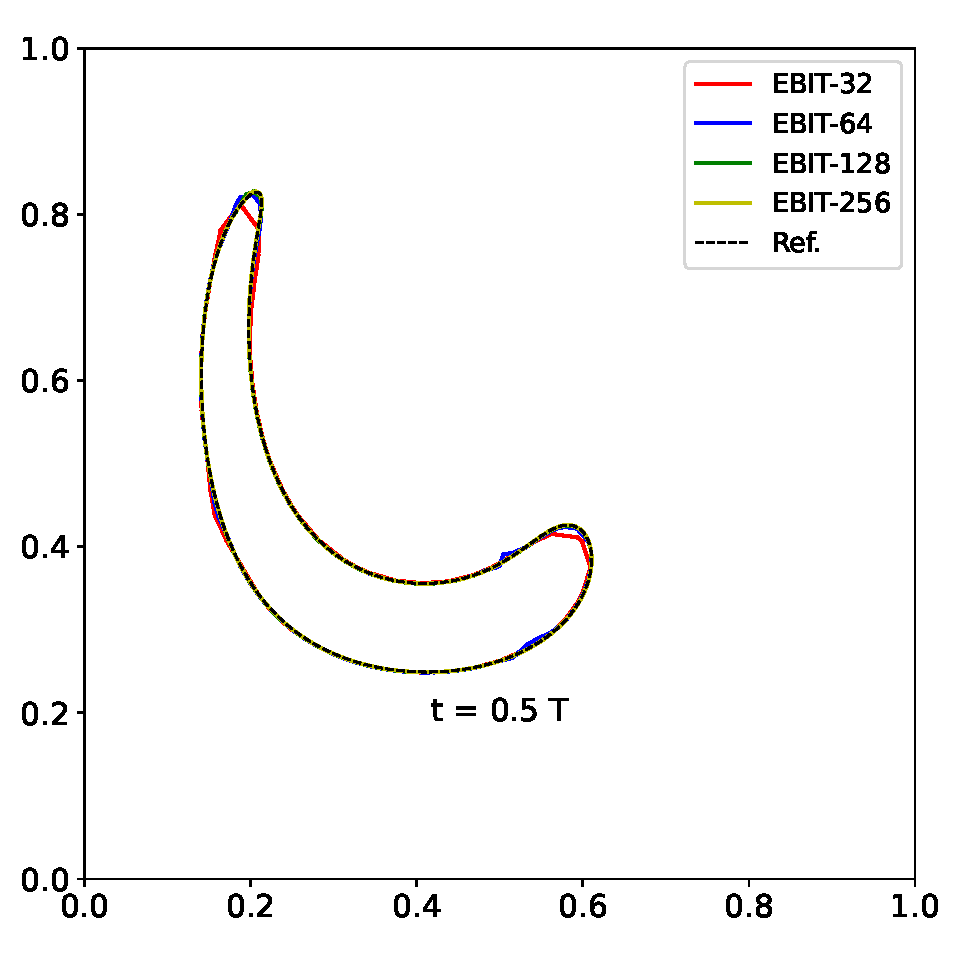
\includegraphics[width=0.45\textwidth]{vortex_intf_2_1} &
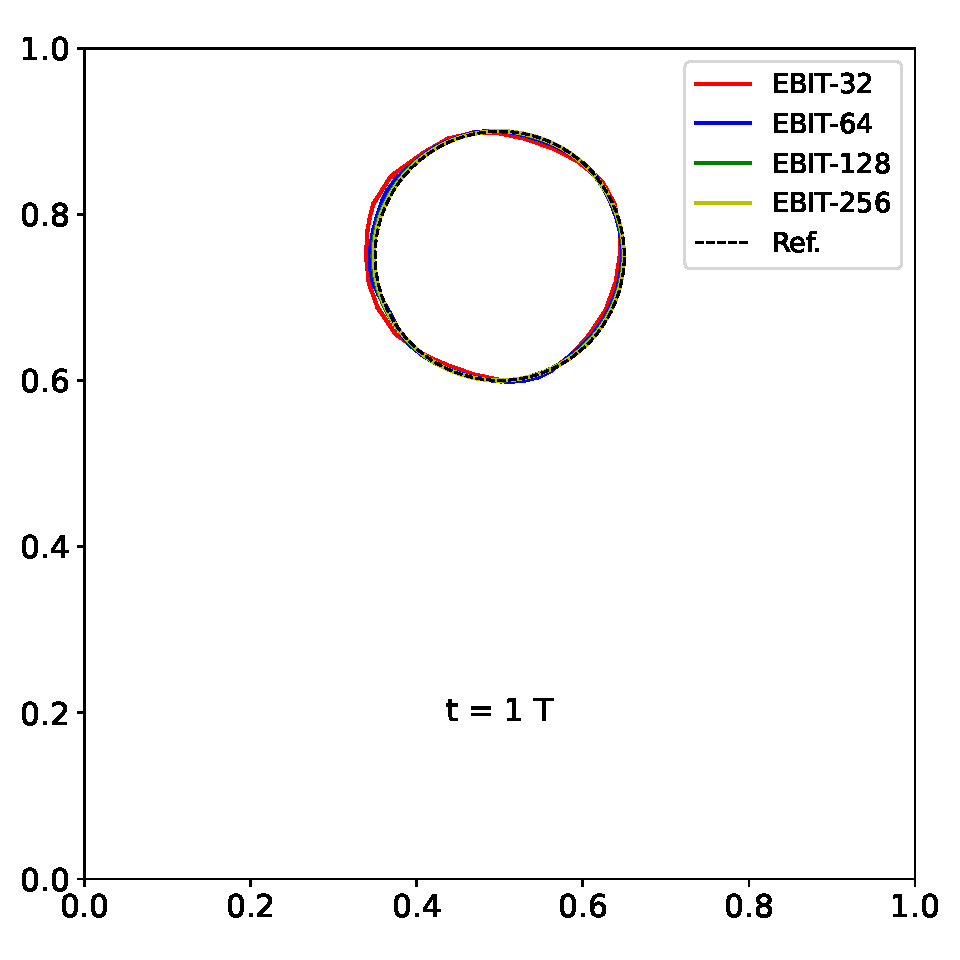
\includegraphics[width=0.45\textwidth]{vortex_intf_2_2}\\
(a) & (b) 
\end{tabular}
\end{center}
\caption{Single vortex test with period $T = 2$ at different resolutions: (a) interface lines at halftime; (b) interface lines at the end of the simulation.}
\label{Fig_vortex_intf_t2}
\end{figure}
% ----------
\begin{figure}
\begin{center}
\begin{tabular}{cc}
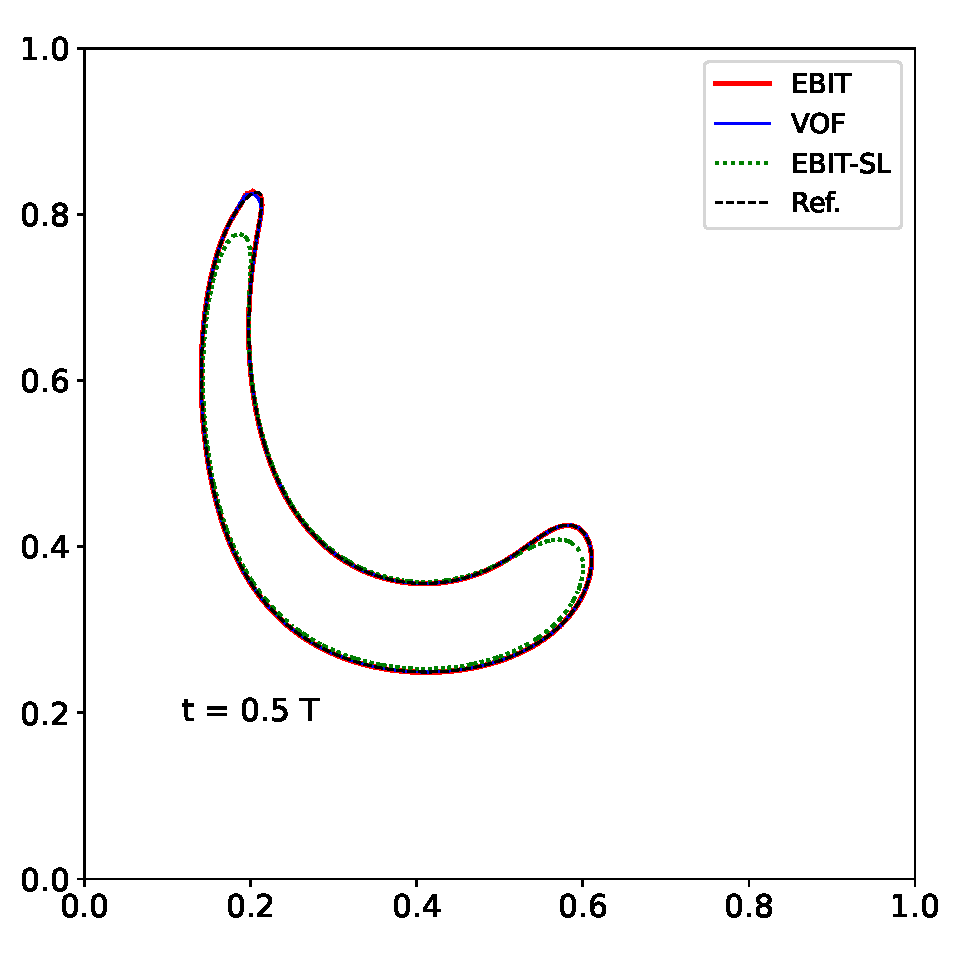
\includegraphics[width=0.45\textwidth]{vortex_intf_vof_2_1} &
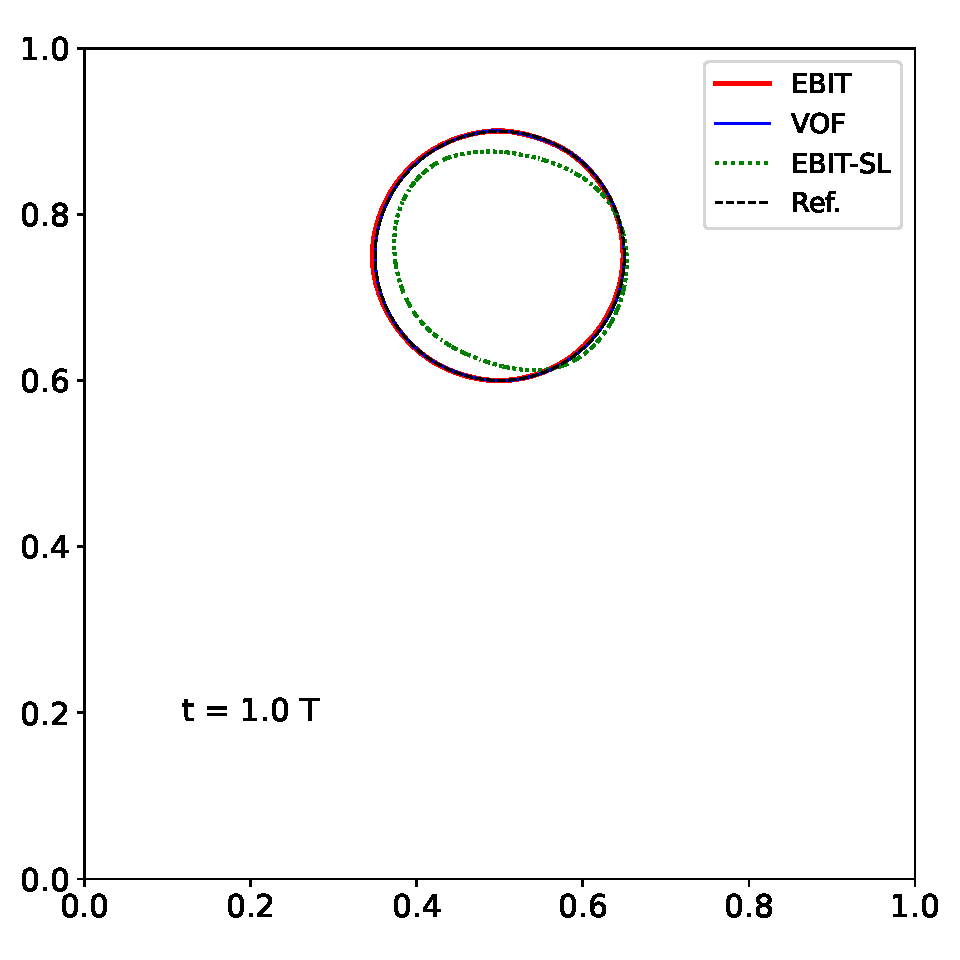
\includegraphics[width=0.45\textwidth]{vortex_intf_vof_2_2}\\
(a) & (b) 
\end{tabular}
\end{center}
\caption{Single vortex test with period $T = 2$ at resolution $N_x = 128$ with different methods: (a) interface lines at halftime; (b) interface lines at the end of the simulation.}
\label{Fig_vortex_intf_t2_cmp}
\end{figure}
% ----------
\begin{table}[hbt!]
\footnotesize
\caption{Mesh convergence study for the single vortex test with period $T = 2$.}
\centering
\begin{tabular}{cc|cccccc}
\hline 
 &$N_x$& 32 & 64 & 128 & 256 & 512 & 1024\\ 
\hline 
EBIT&$E_{area}$ & $1.69\times 10^{-2}$ & $7.45 \times 10^{-3}$ & $2.62 \times 10^{-3}$ & $1.25 \times 10^{-3}$ & $5.99 \times 10^{-4}$ & $2.87 \times 10^{-4}$\\ 
&$E_{shape}$ & $1.45 \times 10^{-2}$ & $6.74 \times 10^{-3}$ & $3.07 \times 10^{-3}$ & $1.54 \times 10^{-3}$ & $7.75 \times 10^{-4}$ & $3.85 \times 10^{-4}$\\
&$E_{sym}$ & $4.59 \times 10^{-3}$ & $2.16 \times 10^{-3}$ & $1.06 \times 10^{-3}$ & $5.28 \times 10^{-4}$ & $2.62 \times 10^{-4}$ & $1.31 \times 10^{-4}$\\
\hline
VOF &$E_{shape}$ & $8.79 \times 10^{-3}$ & $3.00 \times 10^{-3}$ & $1.17 \times 10^{-3}$ & $4.11 \times 10^{-4}$ & $1.21 \times 10^{-4}$ & $3.38 \times 10^{-5}$\\
&$E_{sym}$ & $3.16 \times 10^{-3}$ & $6.93 \times 10^{-4}$ & $1.43 \times 10^{-4}$ & $3.14 \times 10^{-5}$ & $7.48 \times 10^{-6}$ & $2.11 \times 10^{-6}$\\
\hline 
EBIT-SL &$E_{area}$ & $8.26\times 10^{-1}$ & $3.66 \times 10^{-1}$ & $1.71 \times 10^{-1}$ & $8.19 \times 10^{-2}$ & $4.02 \times 10^{-2}$ & $1.99 \times 10^{-2}$\\ 
&$E_{shape}$ & $1.20 \times 10^{-1}$ & $5.77 \times 10^{-2}$ & $2.68 \times 10^{-2}$& $1.33 \times 10^{-2}$ & $6.99 \times 10^{-3}$ & $3.77 \times 10^{-3}$\\
&$E_{sym}$ & $5.80 \times 10^{-2}$ & $2.80 \times 10^{-2}$ & $1.38 \times 10^{-2}$& $6.82 \times 10^{-3}$ & $3.38 \times 10^{-3}$ & $1.69 \times 10^{-3}$\\
\hline 
\end{tabular}
\label{Tab_vortex_error_t2}
\normalsize
\end{table}
% ----------
\begin{figure}
\begin{center}
\begin{tabular}{ccc}
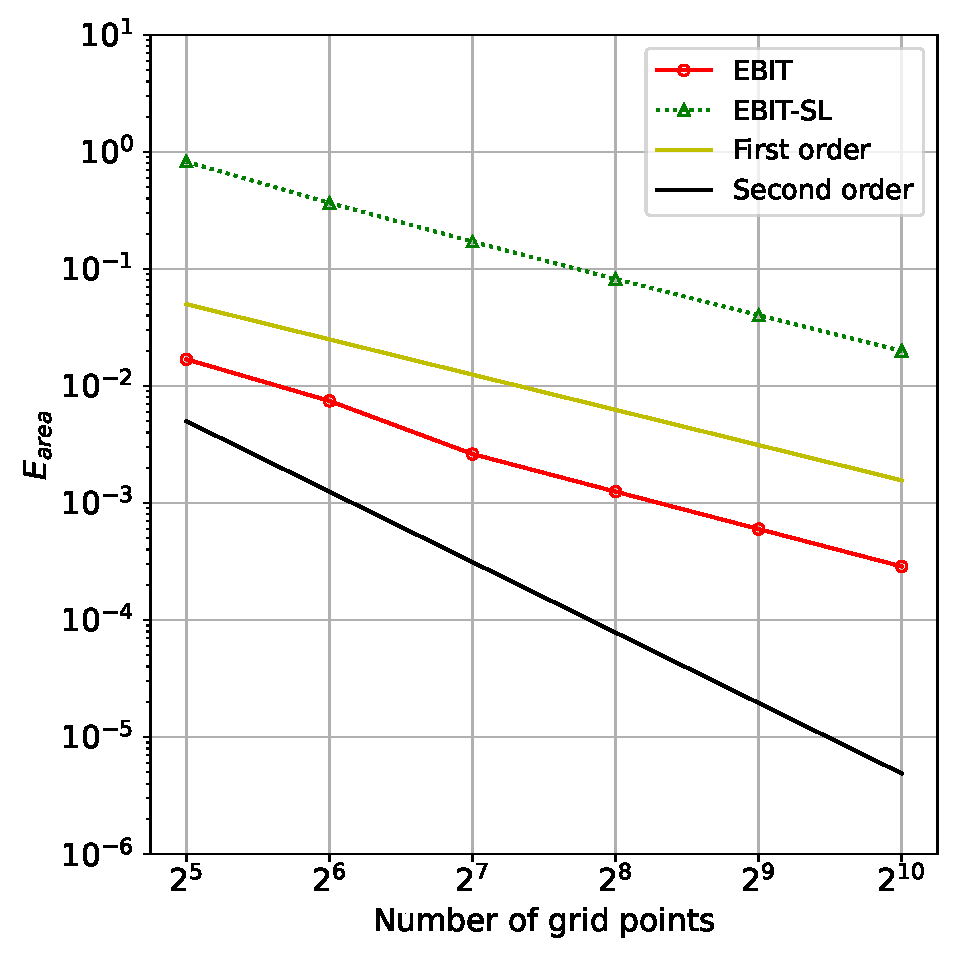
\includegraphics[width=0.33\textwidth]{vortex_err_area_t2} &
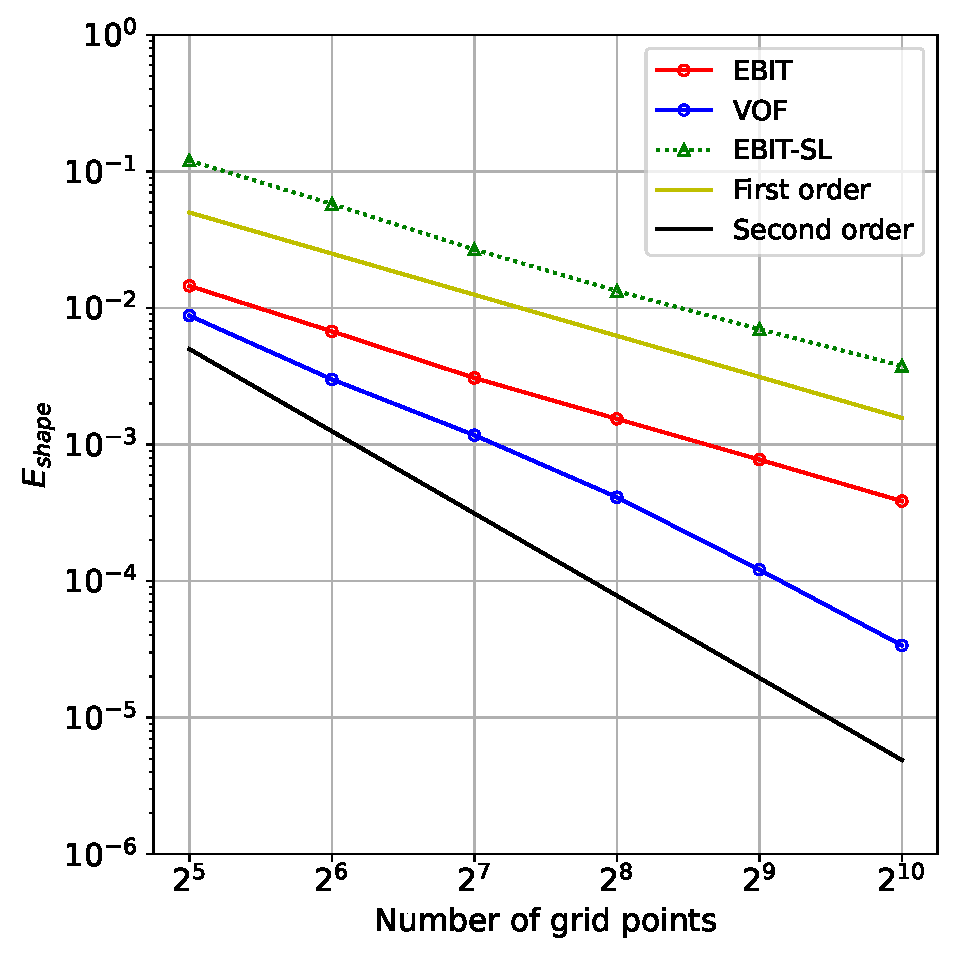
\includegraphics[width=0.33\textwidth]{vortex_err_shape_t2} &
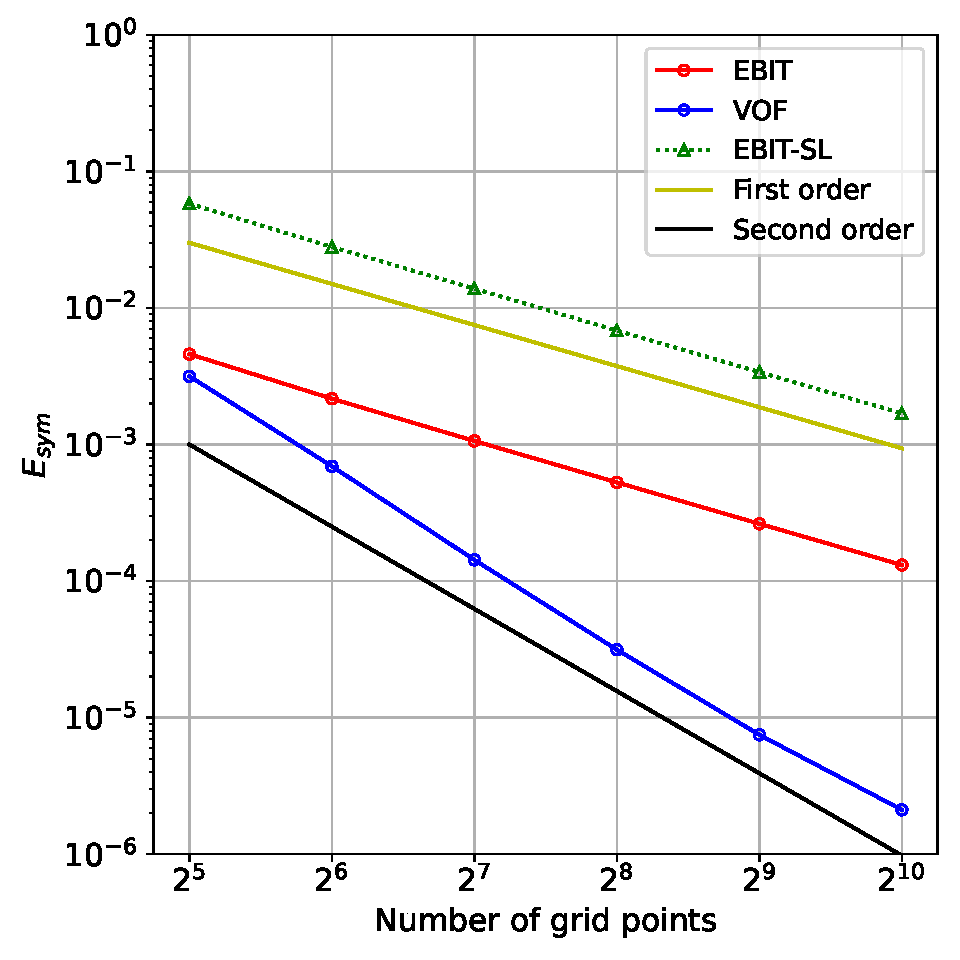
\includegraphics[width=0.33\textwidth]{vortex_err_sym_t2}\\
(a) & (b) & (c)
\end{tabular}
\end{center}
\caption{Errors in the single vortex test with period $T=2$ for different methods as a function of grid resolution: (a) area error $E_{area}$; (b) shape error $E_{shape}$; (c) symmetric difference error $E_{sym}$.}
\label{Fig_vortex_error_t2}
\end{figure}
% ----------

The interface line at maximum deformation and back to its initial position, for the test with period $T = 2$, is shown in Fig.~\ref{Fig_vortex_intf_t2} for different mesh resolutions. Even at the lowest resolution $N_x = 32$, with the new EBIT method we still recover the initial shape and lose little mass. 
The interface line obtained with different methods is shown in Fig.~\ref{Fig_vortex_intf_t2_cmp} for the resolution $N_x = 128$. The results obtained with the new EBIT method and the PLIC-VOF method agree rather well with each other. For the EBIT method with a straight line fit, we observe a considerable amount of area loss.

The area error $E_{area}$, the shape error $E_{shape}$ and the symmetric difference error $E_{sym}$ are listed in Table~\ref{Tab_vortex_error_t2} and are shown in Fig.~\ref{Fig_vortex_error_t2} for the different methods here considered. For the new EBIT method that implements a circle fit, a first-order convergence rate is observed for both errors. The shape errors calculated with the new EBIT method converge less fast than those with the PLIC-VOF method. For the PLIC-VOF method, a second-order convergence rate is observed for the symmetric difference errors, which is higher than that of the shape error.

% ----------
\begin{figure}
\begin{center}
\begin{tabular}{cc}
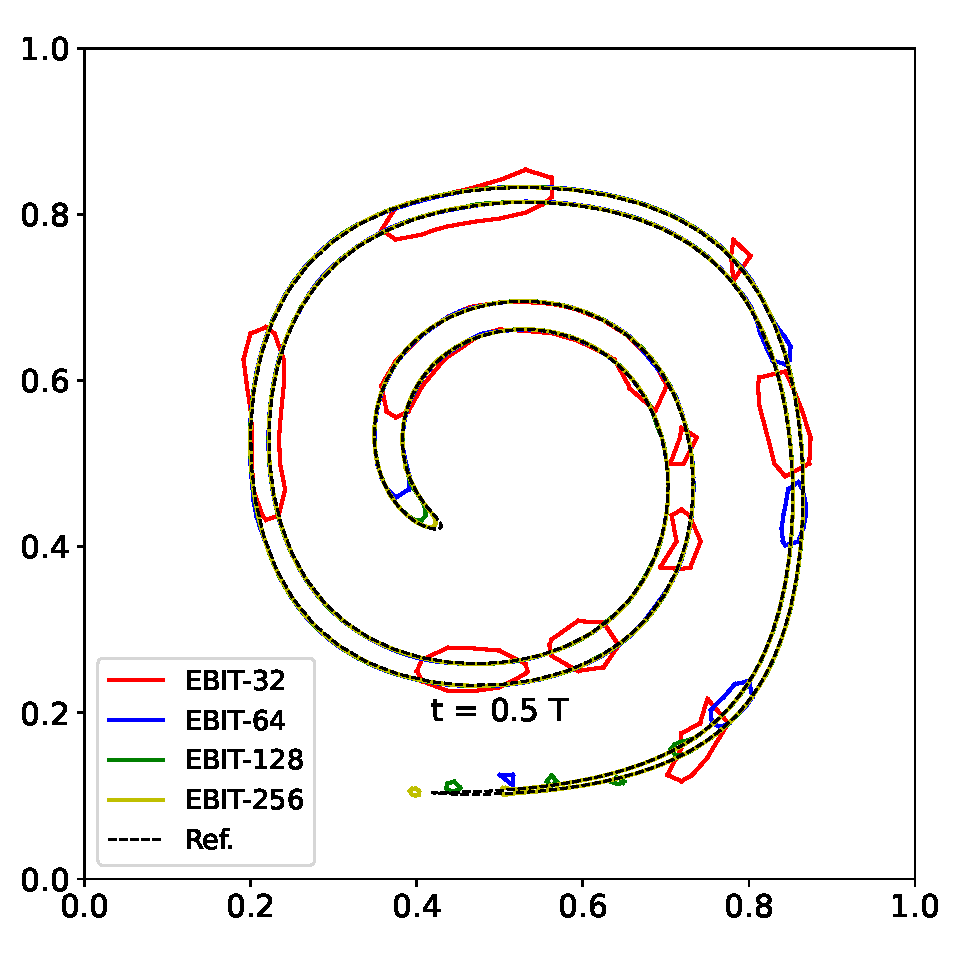
\includegraphics[width=0.45\textwidth]{vortex_intf_8_1} &
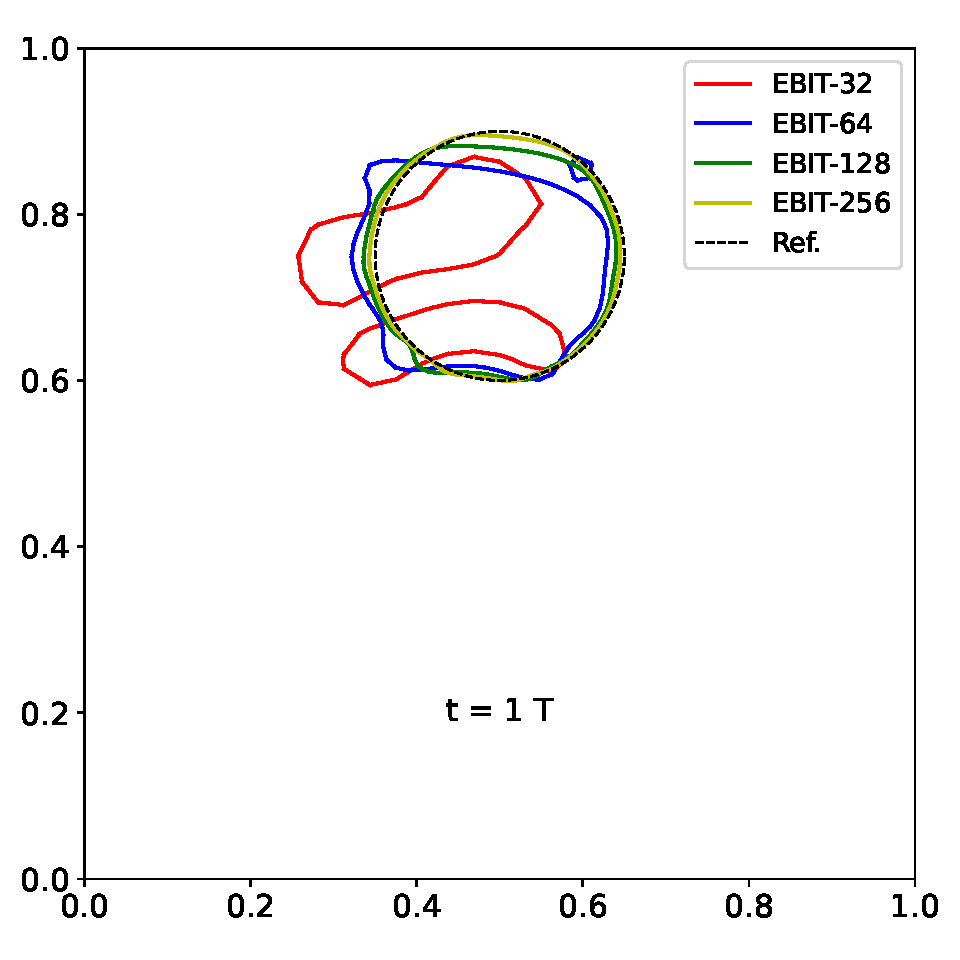
\includegraphics[width=0.45\textwidth]{vortex_intf_8_2}\\
(a) & (b)
\end{tabular}
\end{center}
\caption{Single vortex test with period $T = 8$ at different resolutions: (a) interface lines at halftime; (b) interface lines at the end of the simulation.}
\label{Fig_vortex_intf_t8}
\end{figure}
% ----------
\begin{figure}
\begin{center}
\begin{tabular}{cc}
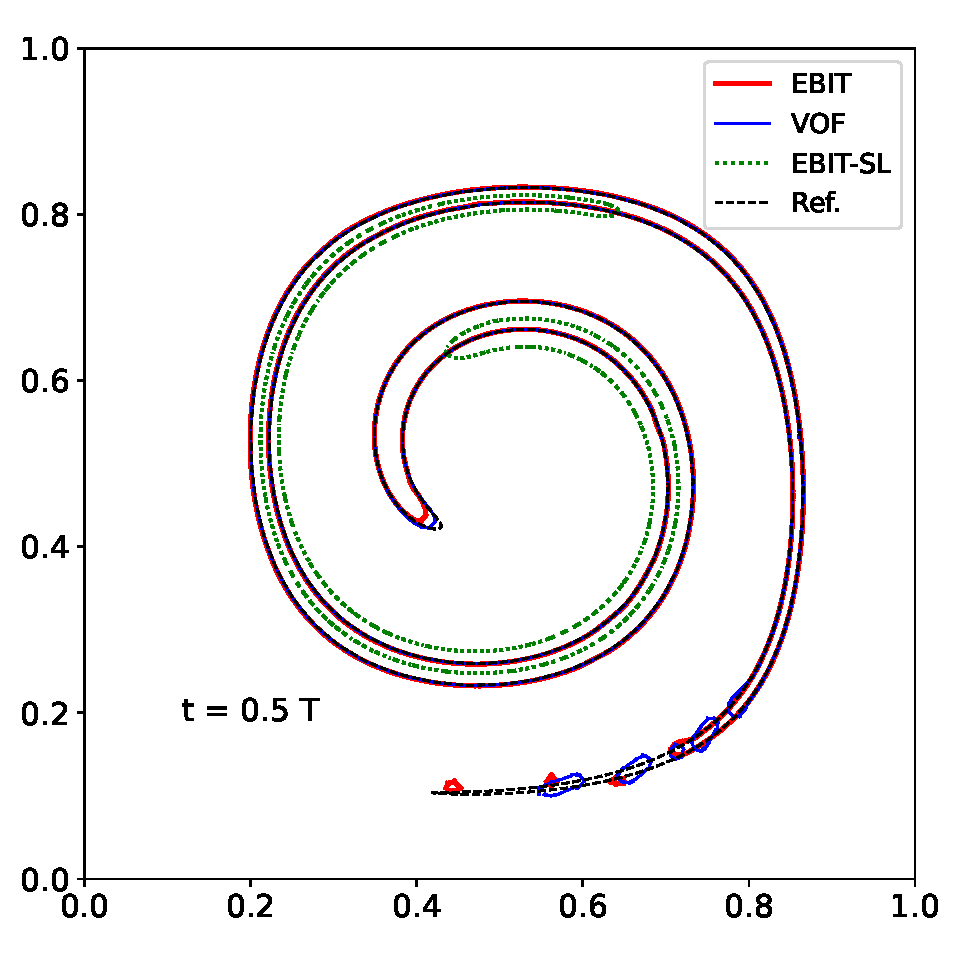
\includegraphics[width=0.45\textwidth]{vortex_intf_vof_8_1} &
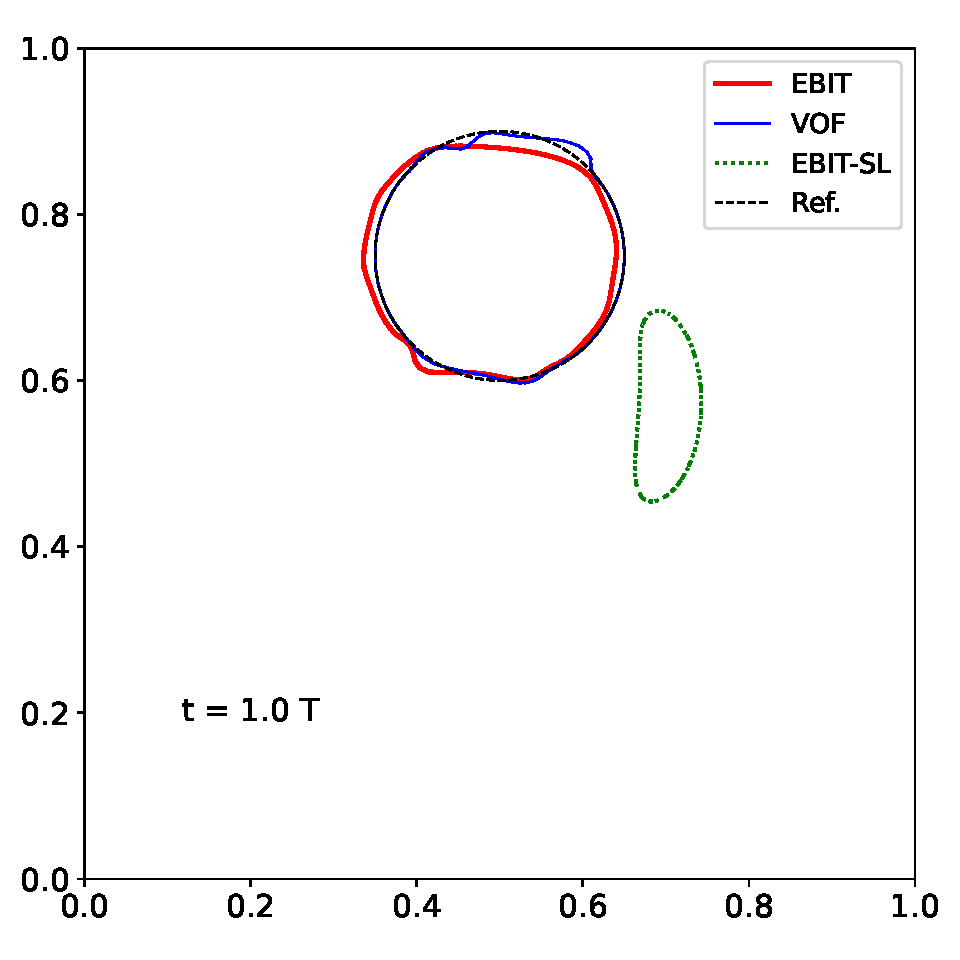
\includegraphics[width=0.45\textwidth]{vortex_intf_vof_8_2}\\
(a) & (b) 
\end{tabular}
\end{center}
\caption{Single vortex test with period $T = 8$ at resolution $N_x = 128$ with different
methods: (a) interface lines at halftime; (b) interface lines at the end of the simulation.}
\label{Fig_vortex_intf_t8_cmp}
\end{figure}
% ----------
\begin{table}[hbt!]
\footnotesize
\caption{Mesh convergence study for the single vortex test with period $T = 8$.}
\centering
\begin{tabular}{cc|ccccc}
\hline 
 &$N_x$& 32 & 64 & 128 & 256 & 512\\ 
\hline 
EBIT &$E_{area}$ & $3.80 \times 10^{-1}$ & $7.71 \times 10^{-2}$ & $2.43 \times 10^{-2}$ & $2.32 \times 10^{-3}$ & $8.23 \times 10^{-5}$\\ 
&$E_{shape}$ & $1.47 \times 10^{-1}$ & $4.99 \times 10^{-2}$ & $2.09 \times 10^{-2}$ & $7.07 \times 10^{-3}$ & $3.54 \times 10^{-3}$\\
&$E_{sym}$ & $4.13 \times 10^{-2}$ & $2.11 \times 10^{-2}$ & $8.09 \times 10^{-3}$ & $3.27 \times 10^{-3}$ & $1.56 \times 10^{-3}$\\
\hline 
VOF &$E_{shape}$ & $2.57 \times 10^{-1}$ & $6.58 \times 10^{-2}$ & $1.35 \times 10^{-2}$ & $7.67 \times 10^{-3}$ & $1.34 \times 10^{-3}$\\
&$E_{sym}$ & $7.01 \times 10^{-2}$ & $1.58 \times 10^{-2}$ & $1.95 \times 10^{-3}$ & $6.02 \times 10^{-4}$ & $1.03 \times 10^{-4}$\\
\hline 
EBIT-SL &$E_{area}$ & NA & NA & $7.98 \times 10^{-1}$ & $ 3.55 \times 10^{-1}$ & $ 1.61 \times 10^{-1}$\\ 
&$E_{shape}$ & NA & NA & $2.02 \times 10^{-1}$ & $1.29 \times 10^{-1}$ & $8.53 \times 10^{-2}$\\
&$E_{sym}$ & NA & NA & $8.49 \times 10^{-2}$ & $7.24 \times 10^{-2}$ & $4.07 \times 10^{-2}$\\
\hline 
\end{tabular}
\label{Tab_vortex_error_t8}
\normalsize
\end{table}
% ----------

The interface line at maximum deformation and back to its initial position, for the test with period $T = 8$ is shown in Fig.~\ref{Fig_vortex_intf_t8} for different mesh resolutions. In this test, the interface line at maximum deformation at halftime
is stretched into a long thin ligament. When the mesh resolution is too coarse, i.e. $N_x = 32$, the new EBIT method loses some mass due to the artificial topological change mechanism. As the mesh resolution is increased, the mass loss progressively decreases and the method recovers better and better the initial circular shape.

The interface line obtained with different methods is shown in Fig.~\ref{Fig_vortex_intf_t8_cmp} for the resolution $N_x = 128$. At this intermediate mesh resolution, there is some discrepancy between the final shape obtained with the new EBIT method and that with the PLIC-VOF method. However, they show the same level of deviation from the reference solution. 

For the EBIT method with a straight line fit, there is an even more pronounced mass loss. Furthermore, the interface does not return to its initial position due to the lateral shift of the interface with respect to the reference solution, as shown in Fig.~\ref{Fig_vortex_intf_t8_cmp}a at maximum deformation.

% ----------
\begin{figure}
\begin{center}
\begin{tabular}{ccc}
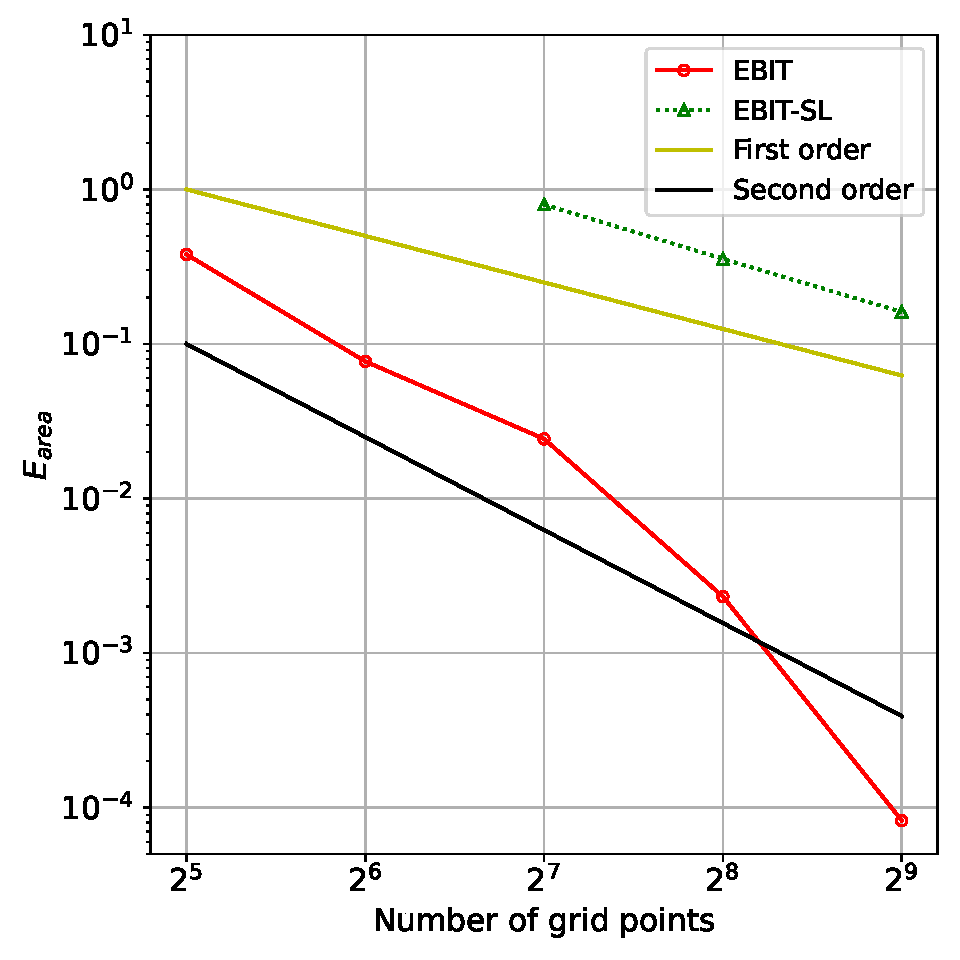
\includegraphics[width=0.33\textwidth]{vortex_err_area_t8} &
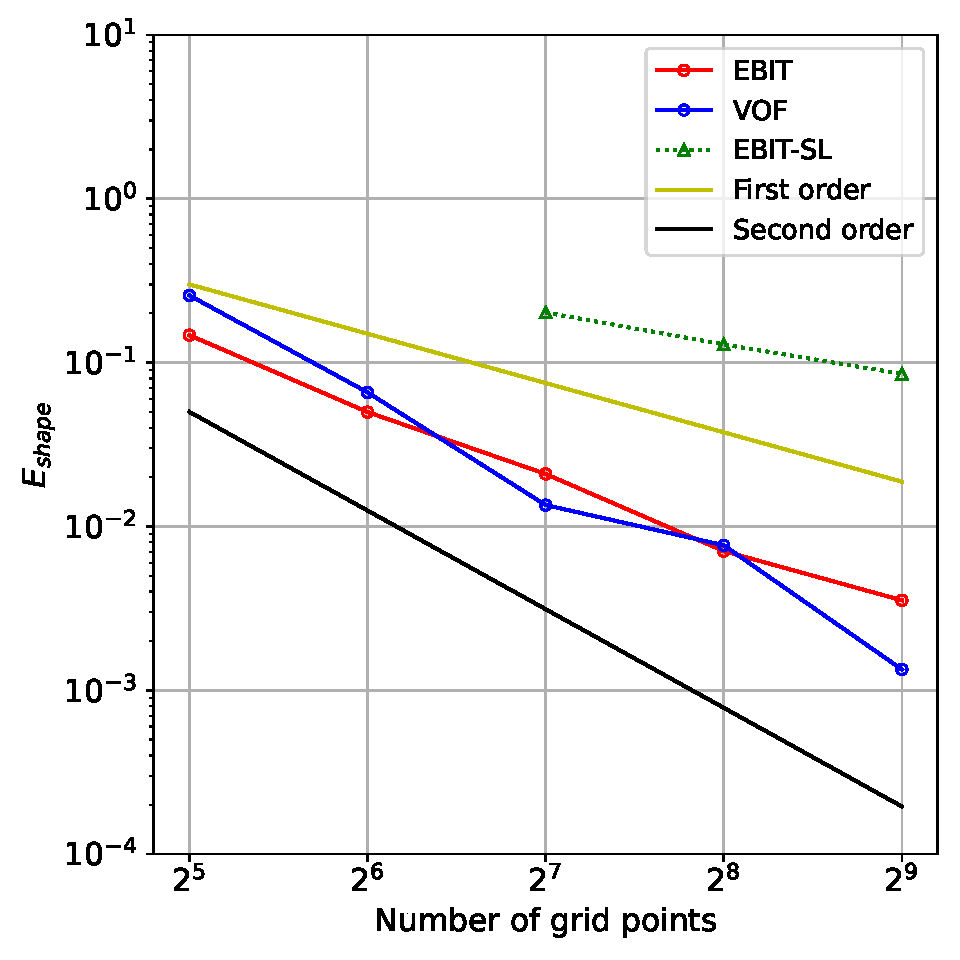
\includegraphics[width=0.33\textwidth]{vortex_err_shape_t8}&
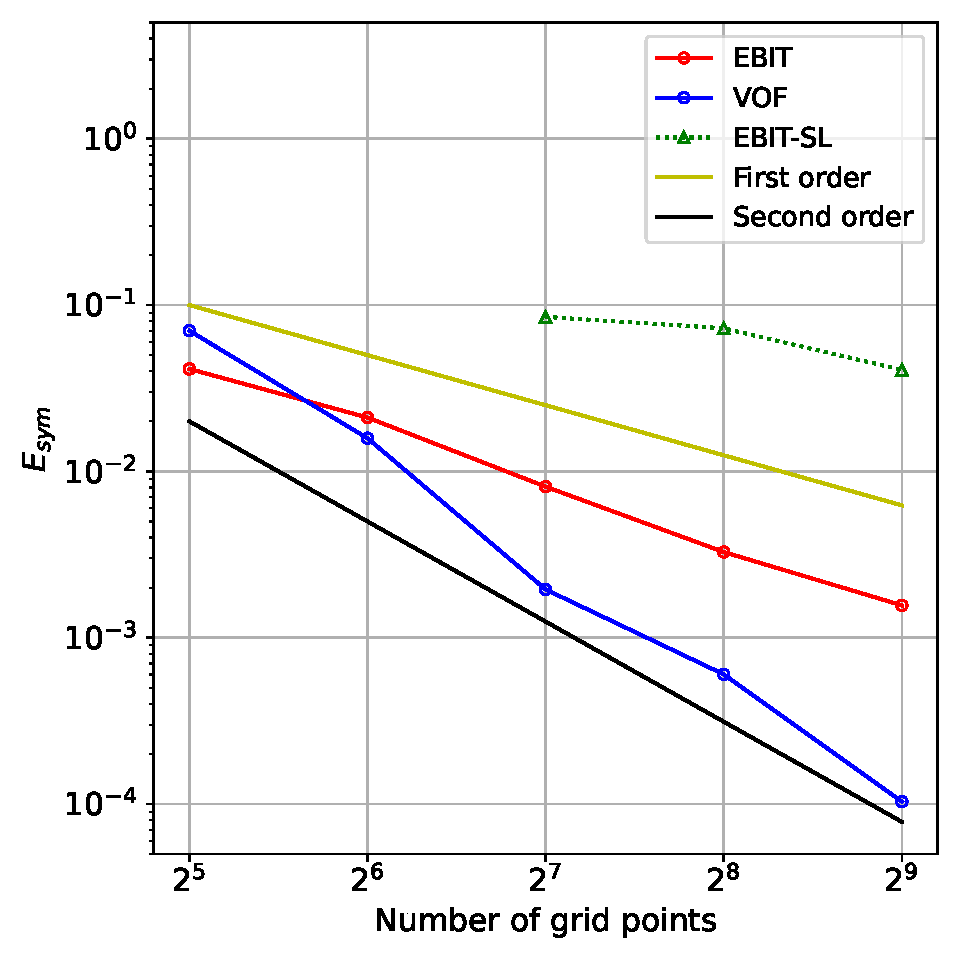
\includegraphics[width=0.33\textwidth]{vortex_err_sym_t8}\\
(a) & (b) & (c)
\end{tabular}
\end{center}
\caption{Errors in the single vortex test with period $T = 8$ for different methods as a function of grid resolution: (a) area error $E_{area}$; (b) shape error $E_{shape}$; (c) symmetric difference error $E_{sym}$.}
\label{Fig_vortex_error_t8}
\end{figure}
% ----------

The area error $E_{area}$, the shape error $E_{shape}$ and the symmetric difference error $E_{sym}$ are listed in Table~\ref{Tab_vortex_error_t8} and are shown in Fig.~\ref{Fig_vortex_error_t8}. For the new EBIT method, a convergence rate between first-order and second-order is observed for the area and shape errors, but only a  first-order convergence rate is observed for the symmetric difference error. This behavior is similar to that obtained in the previous test with period $T=2$. The shape errors obtained with the new EBIT method and the PLIC-VOF method become closer to each other as the mesh is refined. A second-order convergence rate is still observed for the symmetric difference error calculated with the PLIC-VOF method.
The EBIT method with a straight line fit loses all the reference phase even when an intermediate mesh resolution, $N_x = 64$, is used.
All the kinematic tests show that the new EBIT method with a circle fit does decrease the mass loss as the interface is reconstructed, thus increasing the accuracy of mass conservation.

In order to demonstrate the feasibility of the integration of the new EBIT method with AMR, we run again the single-vortex test case on a quadtree grid in Basilisk. The interface lines at halftime and at the end of the simulation and the corresponding meshes are shown in Fig.~\ref{Fig_vortex_intf_t8_amr}. The maximum level of refinement is $N_{l,max}=7$, which corresponds to the mesh resolution $N_x =128$, while the minimum level is $N_{l,min}=4$. All the cells near the interface are refined to the maximum level, to avoid an inconsistency like that shown in Fig.~\ref{Fig_ebit_amr}. Since the applied velocity field is not affected by the mesh resolution and the same stencil is used for the velocity interpolation, the interface line obtained on the quadtree grid coincides with that on the fixed Cartesian mesh.
% ----------
\begin{figure}
\begin{center}
\begin{tabular}{cc}
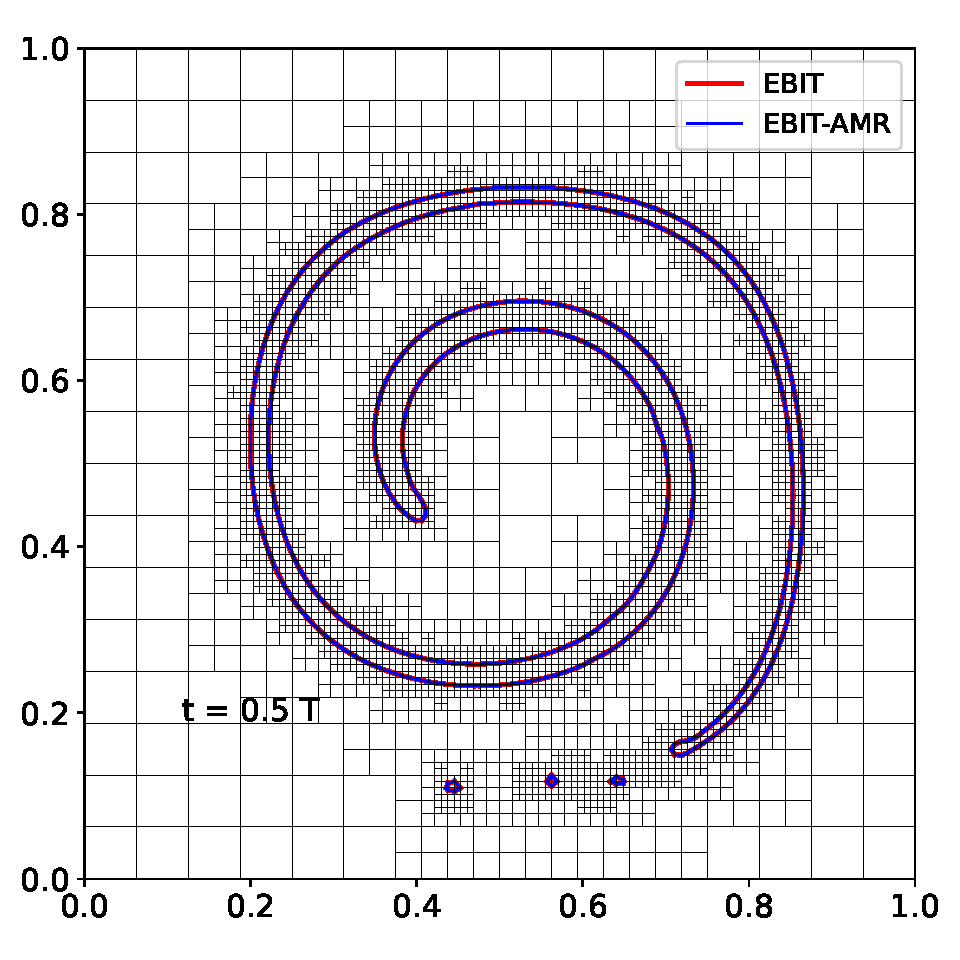
\includegraphics[width=0.45\textwidth]{vortex_intf_amr_8_1} &
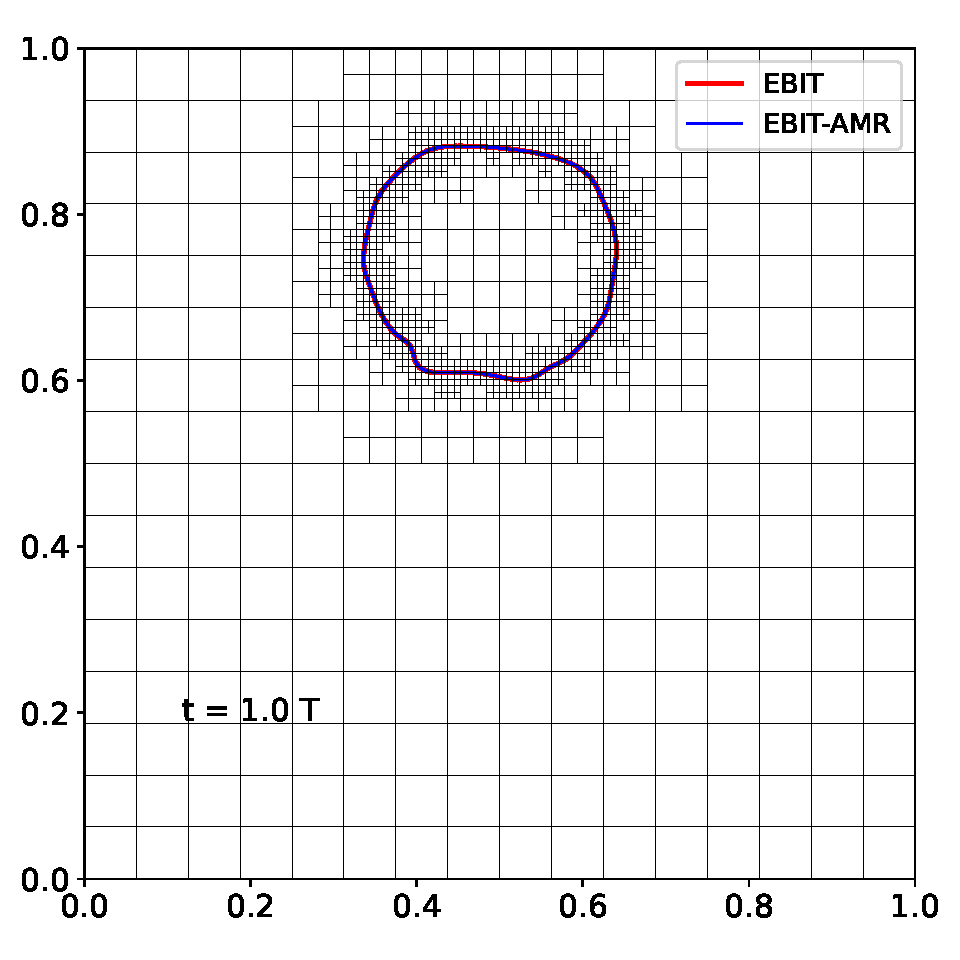
\includegraphics[width=0.45\textwidth]{vortex_intf_amr_8_2}\\
(a) & (b) 
\end{tabular}
\end{center}
\caption{Single vortex test with period $T = 8$ at fixed resolution $N_x=128$ and AMR with $N_{l,max}=7$ and $N_{l,min}=4$: (a) interface lines at halftime; (b) interface lines at the end of the simulation.}
\label{Fig_vortex_intf_t8_amr}
\end{figure}
% ----------

\subsection{Zalesak's disk}

The Zalesak's disk \cite{Zalesak_1979_31} test case is used to assess the ability of the EBIT method to deal with sharp edges and corners. A notched circular interface of radius $R = 0.15$ and center at $(0.5, 0.75)$ is placed inside the unit square domain. The notched width is $0.05$ and its length $0.25$. A constant velocity field, $(u, v) = (2\pi (0.5 - y), 2\pi (x - 0.5))$, is applied, so that the interface performs a rotation around the center of the computational domain and returns to its initial position at $t = T = 1.0$.

In the simulations we use a constant timestep that varies with the mesh resolution. Its value is determined by the maximum velocity at time $t=0$ so that $CFL = u_{max} \Delta t / \Delta = \pi / 16 \approx 0.2$. The error is again measured by the area and symmetric difference errors.

The interface line at the end of the simulation is shown in Fig.~\ref{Fig_zalesak_intf}a for different mesh resolutions. The new EBIT method retains rather well the circular section of the interface for all mesh resolutions, except near the corners of the notch. As the mesh resolution is increased, the lateral sides of the notch are better approximated by the new EBIT method, while the interface smoothing near the corners progressively decreases.

The interface line obtained with different methods is shown in Fig.~\ref{Fig_zalesak_intf}b for the resolution $N_x = 128$. For the EBIT method with a straight line fit, the whole notched region has disappeared at the end of the simulation and there is also a relevant mass loss. The new EBIT method and the PLIC-VOF method present a similar level of smoothing near the four corner regions.

% ----------
\begin{figure}
\begin{center}
\begin{tabular}{cc}
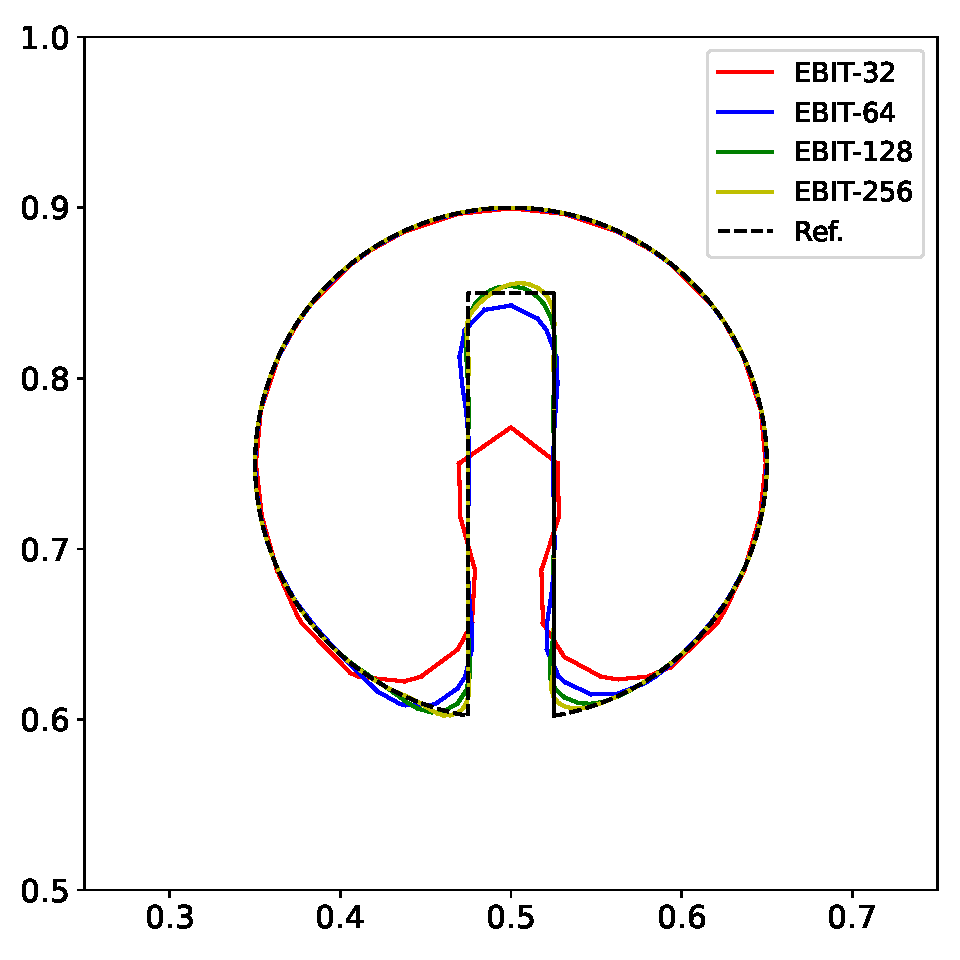
\includegraphics[width=0.45\textwidth]{zalesak_intf} &
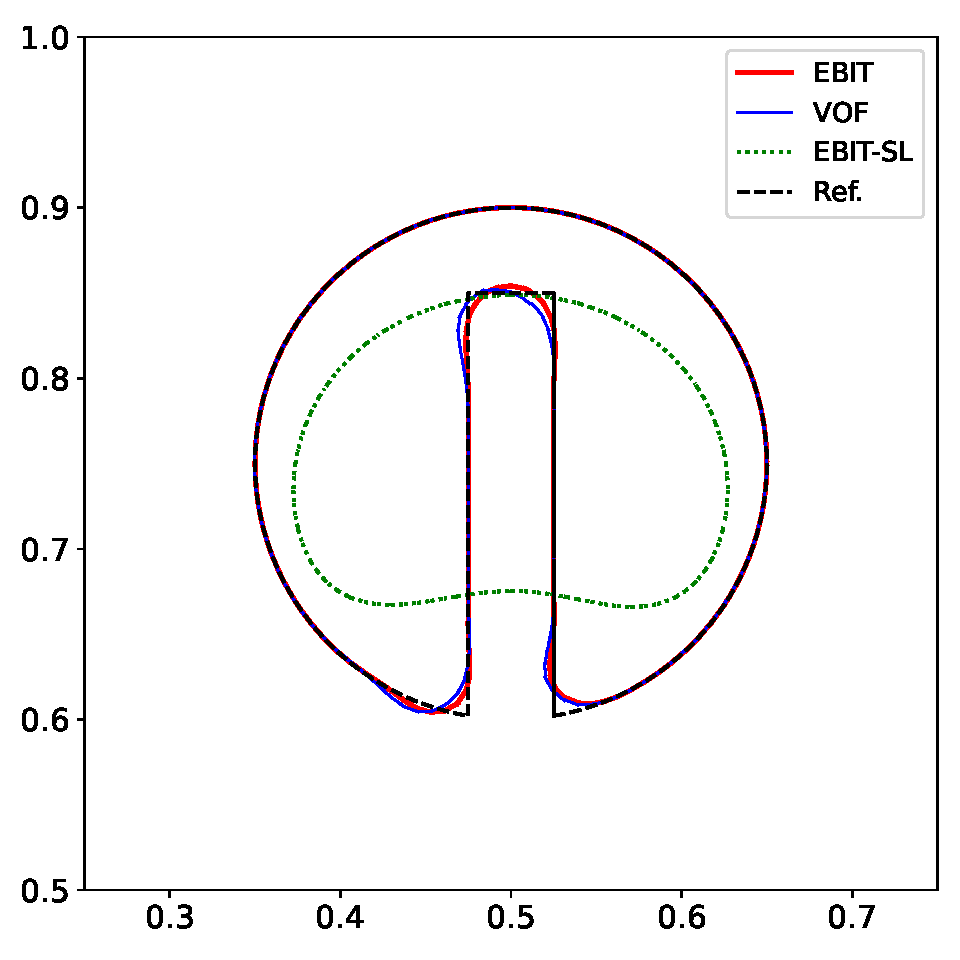
\includegraphics[width=0.45\textwidth]{zalesak_intf_vof}\\
(a) & (b) 
\end{tabular}
\end{center}
\caption{Zalesak's disk, interface lines at the end of the simulation: (a) interface lines for different mesh resolutions; (b) interface lines with different methods ($N_x = 128$).}
\label{Fig_zalesak_intf}
\end{figure}
% ----------

% ----------
\begin{figure}
\begin{center}
\begin{tabular}{cc}
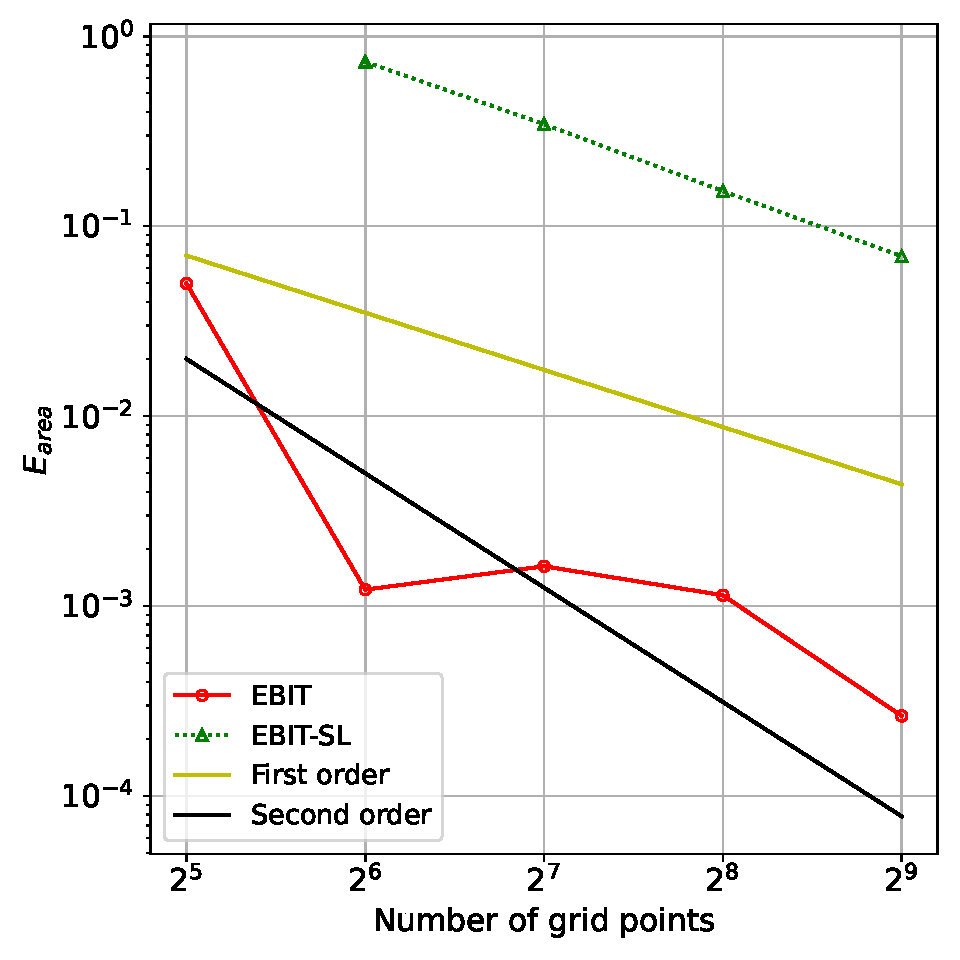
\includegraphics[width=0.45\textwidth]{zalesak_err_area} &
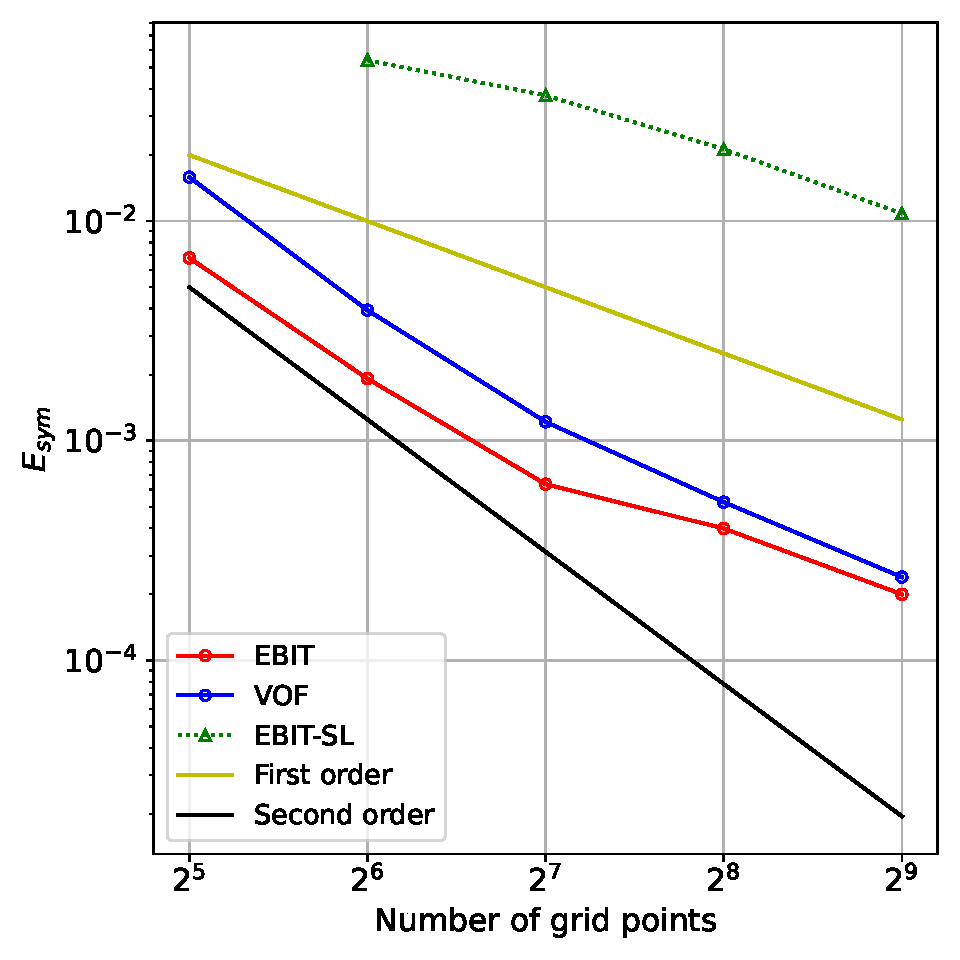
\includegraphics[width=0.45\textwidth]{zalesak_err_sym}\\
(a) & (b)
\end{tabular}
\end{center}
\caption{Errors in the Zalesak's disk test for different methods as a function of grid resolution: (a) area error $E_{area}$; (b) symmetric difference error $E_{sym}$.}
\label{Fig_zalesak_error}
\end{figure}
% ----------

% ----------
\begin{table}[hbt!]
\footnotesize
\caption{Mesh convergence study for the Zalesak's disk test.}
\centering
\begin{tabular}{cc|ccccc}
\hline 
 &$N_x$& 32 & 64 & 128 & 256 & 512\\ 
\hline 
EBIT &$E_{area}$ & $4.99 \times 10^{-2}$ & $1.22 \times 10^{-3}$ & $1.62 \times 10^{-3}$ & $1.14 \times 10^{-3}$ & $2.64 \times 10^{-4}$\\ 
&$E_{sym}$ & $6.80 \times 10^{-3}$ & $1.92 \times 10^{-3}$ & $6.35 \times 10^{-4}$ & $3.99 \times 10^{-4}$ & $2.00 \times 10^{-4}$\\
\hline 
VOF & $E_{sym}$ & $1.58 \times 10^{-2}$ & $3.93 \times 10^{-3}$ & $1.22 \times 10^{-3}$ & $5.26 \times 10^{-4}$ & $2.40 \times 10^{-4}$\\
\hline 
EBIT-SL &$E_{area}$ & NA & $7.33 \times 10^{-1}$ & $3.44 \times 10^{-1}$ & $ 1.53 \times 10^{-1}$ & $ 6.94 \times 10^{-2}$\\ 
&$E_{sym}$ & NA & $5.39 \times 10^{-2}$ & $3.73 \times 10^{-2}$ & $2.13 \times 10^{-2}$ & $1.08 \times 10^{-2}$\\
\hline 
\end{tabular}
\label{Tab_zalesak_error}
\normalsize
\end{table}
% ----------

The area error $E_{area}$ and the symmetric difference error $E_{sym}$ are listed in Table~\ref{Tab_zalesak_error} and are shown in Fig.~\ref{Fig_zalesak_error}. For the new EBIT method, the convergence rate of the area error fluctuates at low resolution but it seems to settle down at second-order at the highest resolution. For the PLIC-VOF method, the symmetric difference error presents a convergence rate close to first-order as the resolution is increased. The same error for the new EBIT method is approaching the same behavior but from below. This fact is clearly seen in the shape of the interface lines. Even if the two lines are close to each other, the interface with the new EBIT method is clearly more symmetric with respect to a vertical axis through the notch (see blue and red lines of Fig.~\ref{Fig_zalesak_intf}b).

\subsection{Capillary wave}

Capillary waves are a basic phenomenon of surface-tension-driven flows and their adequate numerical resolution is a prerequisite to more complex applications. The small-amplitude damped oscillations of a capillary wave are now a classical test case to check the accuracy of new numerical schemes that are developed to investigate the evolution in time of viscous, surface-tension-driven two-phase flows.

A sinusoidal perturbation is applied to a plane interface between two fluids initially at rest. Under the influence of surface tension, the interface begins to oscillate around its equilibrium position, while the amplitude of the oscillations decay in time due to viscous dissipation. The exact analytical solution was found by Prosperetti \cite{Prosperetti_1981_24} in the limit of very small amplitudes, and it is usually used as a reference.

In order to get a good agreement with the theory \cite{Popinet_2009_228}, it is necessary to move the top and bottom boundaries far away from the interface, in particular here we consider the rectangular computational domain $[0, \lambda] \times [0, 4 \lambda]$, where $\lambda$ is the wavelength of the perturbation. A symmetric boundary condition is applied on the four sides of the domain. The initial amplitude of the perturbation is 
$\lambda/100$, as in Popinet and Zaleski \cite{Popinet_1999_30}, Denner et al. \cite{Denner_2017_226} and Gerlach et al. \cite{Gerlach_2006_49}. The value of the other physical properties that are used in the simulation and of the Laplace number, 
$La = (\rho_1 \sigma \lambda) \big/ \mu_1^2$, is listed in Table~\ref{Tab_para_capwave}.
In this simulation, the maximum value $CFL = 0.5$ is used. Moreover, the timestep is also limited by the period of the shortest capillary wave:
% ----------
\begin{equation}
\Delta t \leq \frac{(\rho_1 + \rho_2) \Delta^3}{2 \sigma}
\label{Eq_dt_cap}
\end{equation}
% ----------

The time evolution of the maximum amplitude of the interface is shown in Fig.~\ref{Fig_capwave_amp}, together with those of the analytical solution and of the PLIC-VOF method. Time is made dimensionless by using the normal-mode oscillation frequency $\omega_0$, which is defined by the dispersion relation
% ----------
\begin{equation}
\omega_0^2 = \frac{\sigma k^3}{2 \rho_1}
\end{equation}
% ----------
where $k = 2\pi / \lambda$ is the wavenumber and $\lambda = 1$ in our simulation. The numerical results obtained with both the new EBIT and PLIC-VOF methods agree rather well with the analytical solution.

The error between the analytical solution \cite{Prosperetti_1981_24} and the two numerical solutions can be further analyzed with the $L_2$ norm
% ----------
\begin{equation}
E_2 = \frac{1}{\lambda} \sqrt{\frac{\omega_0}{25} \int_{t=0}^{25 / \omega} (h - h_{exact})^2}
\label{Eq_E2}
\end{equation}
% ----------
where $h$ is the maximum interface amplitude obtained with a numerical method
and $h_{exact}$ the reference value. The results are shown in Fig.~\ref{Fig_capwave_acc}
and a convergence rate close to second-order is observed for both methods,
the error of the PLIC-VOF method being always somewhat smaller.
In both simulations, the height function method has been used to calculate the curvature \cite{Popinet_2009_228}. More particularly, since we are considering a very small amplitude of the oscillations, hence of the interface curvature as well, the straight line approximation of the new EBIT method in each cut cell provides a fairly good approximation of the volume fraction and therefore of the calculation of the local height function.

The area error $E_{area}$ of Eq.~\eqref{Eq_error_surface} is used to measure the accuracy of mass conservation in the dynamics test cases. The area $A$ is that occupied by the reference phase. For the simulation at the highest resolution ($N_x \times N_y = 64 \times 256$), $E_{area}$ is $5.3 \times 10^{-6}$.
% ----------
\begin{table}[hbt!]
\caption{Physical properties for the capillary wave test.}
\centering
\begin{tabular}{cccccc}
\hline 
 $\rho_1$ & $\rho_2$ &$\mu_1$ & $\mu_2$ & $\sigma$ & $La$ \\ 
\hline 
$1$ & $1$ &$ 0.01826$& $0.01826$ & $1$ & $3000$ \\ 
\hline 
\end{tabular}
\label{Tab_para_capwave}
\end{table}
% ----------
\begin{figure}
\centering
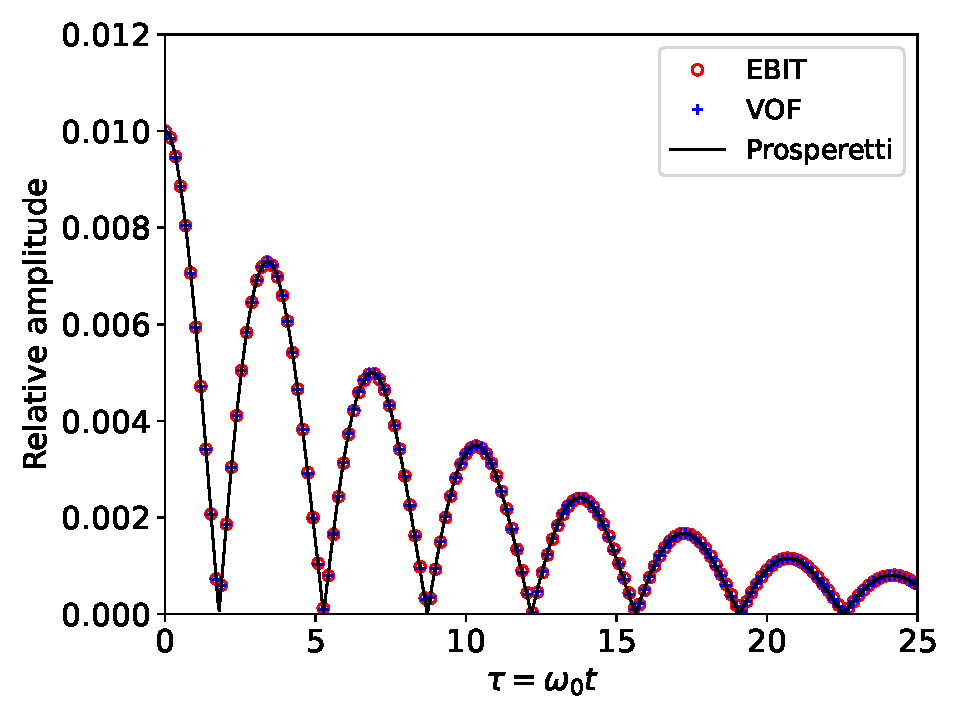
\includegraphics[width=\textwidth]{capwave_amp}
\caption{Capillary wave test with different methods: time evolution of the maximum amplitude of the interface oscillation. The time $\tau = \omega_0\,t$ is non-dimensional and the grid resolution is $N_x \times N_y = 64 \times 256$.}
\label{Fig_capwave_amp}
\end{figure}
% ----------
\begin{figure}
\centering
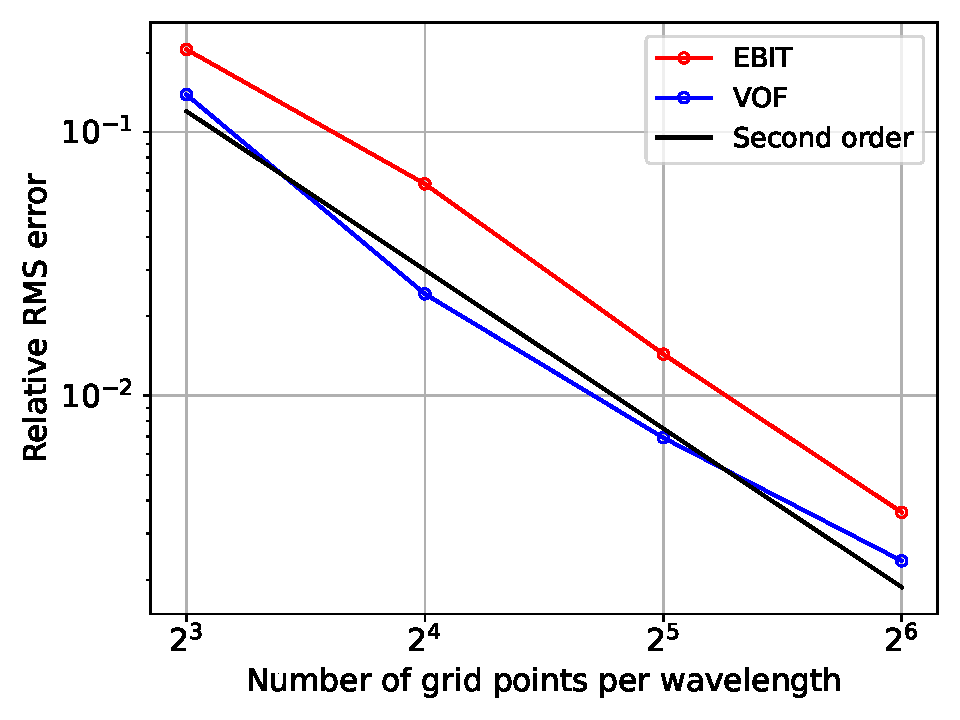
\includegraphics[scale=0.8]{capwave_err}
\caption{Error $E_2$ in the capillary wave test for different methods as a function of the grid resolution.}
\label{Fig_capwave_acc}
\end{figure}
% ----------

\subsection{Rayleigh-Taylor instability}

In order to demonstrate the capability of the new EBIT method to deal with more complex flows, we investigate another classical test: the Rayleigh-Taylor instability at high Reynolds number, that involves a large deformation of the interface. 

The Rayleigh-Taylor instability occurs when a heavy fluid is on top of a lighter one, with the direction of gravity from top to bottom. The density difference between the two fluids plays an important role in the instability and is present in the definition of the dimensionless Atwood number $At$
% ----------
\begin{equation}
At = \frac{\rho_1 - \rho_2}{\rho_1 + \rho_2}
\end{equation}
% ----------
where $\rho_1$ and $\rho_2$ are the densities of the heavy and light fluids, respectively.

This instability has been investigated in several studies \cite{Tryggvason_1988_75, Guermond_2000_165, Ding_2007_226}, that consider an incompressible flow without surface tension effects, with $At = 0.5$ and different Reynolds numbers,
$Re = \big( \rho_1 g^{1/2} d^{3/2} \big) \big/ \mu_1$.

In this study, we consider the rectangular computational domain $[0, d] \times [0, 4d]$, partitioned with $N_x \times N_y = 128 \times 512$ grid cells. The plane interface $y_0(x) = 2\,d$ between the two fluids is perturbed by a sinusoidal wave $y_1(x) = 0.1\,d \cos (k x)$, so that the interface line at the beginning of the simulation is
% ----------
\begin{equation}
y (x) = y_0 (x) + y_1 (x) = 2\,d + 0.1\,d \cos (k x), \quad k = \frac{2\pi}{\lambda}
\end{equation}
% ----------
with $\lambda = d = 1$.
A no-slip boundary condition is enforced at the bottom and at the top of the computational domain, and a symmetric boundary condition on the two vertical sides. 
The value of the other physical properties that are used in the simulation and of the Reynolds number $Re$ is listed in Table~\ref{Tab_para_rti}. In this simulation, the timestep is limited by the $CFL$ number, $CFL=0.05$, and the maximum allowable timestep provided by the user, $\Delta t_{max} = 2 \times 10^{-4}$.

% ----------
\begin{table}[hbt!]
\caption{Physical properties for the Rayleigh-Taylor instability test.}
\centering
\begin{tabular}{cccccc}
\hline 
 $\rho_1$& $ \rho_2$ &$\mu_1$ & $\mu_2$& $g$ & $Re$ \\ 
\hline 
$3 $ & $1$ & $ 0.00313$ & $ 0.00313$& $9.81$ &$3000$ \\ 
\hline 
\end{tabular}
\label{Tab_para_rti}
\end{table}
% ----------
\begin{figure}
\begin{center}
\begin{tabular}{ccc}
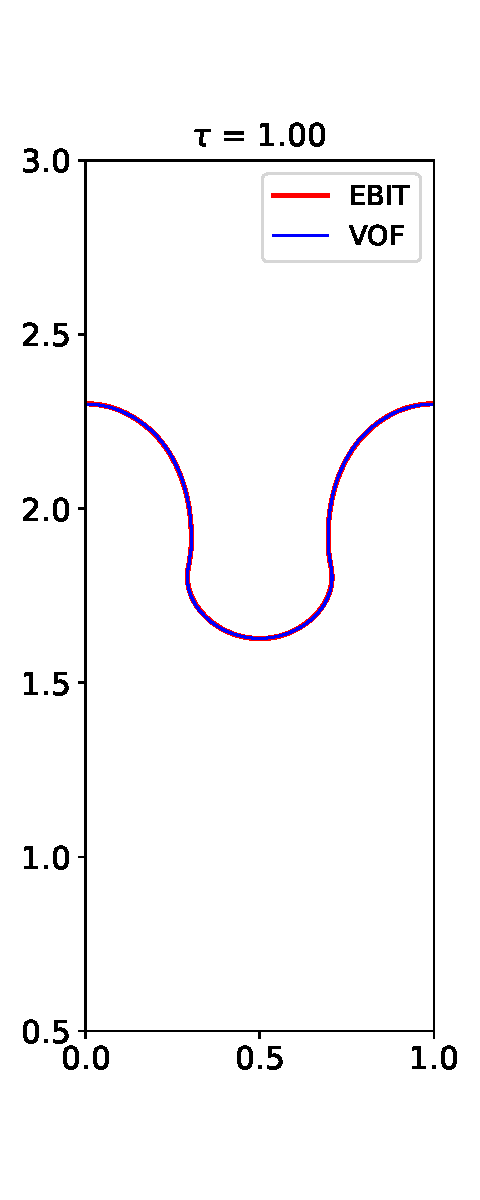
\includegraphics[width=0.25\textwidth]{rti_intf_1} &
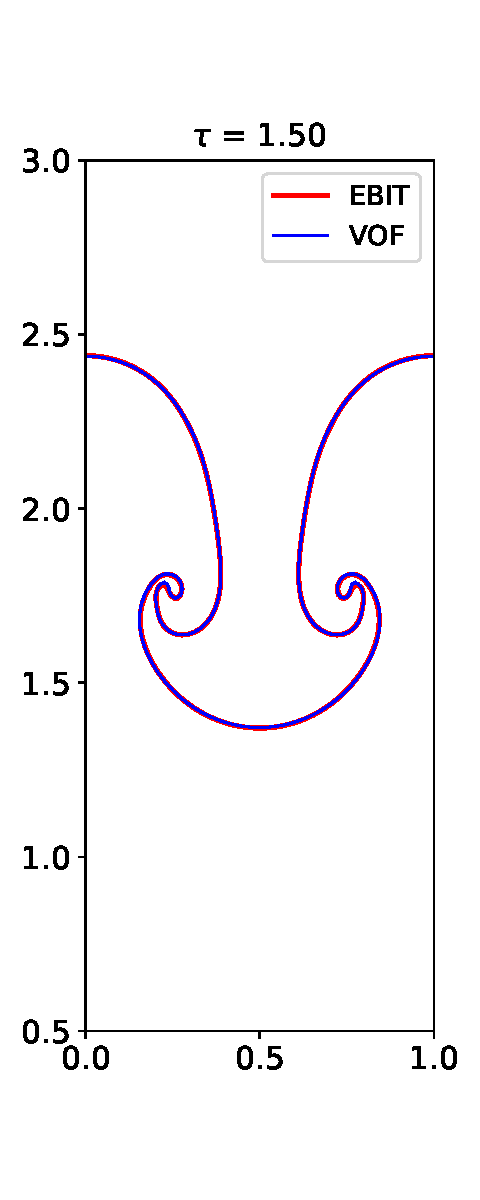
\includegraphics[width=0.25\textwidth]{rti_intf_2} &
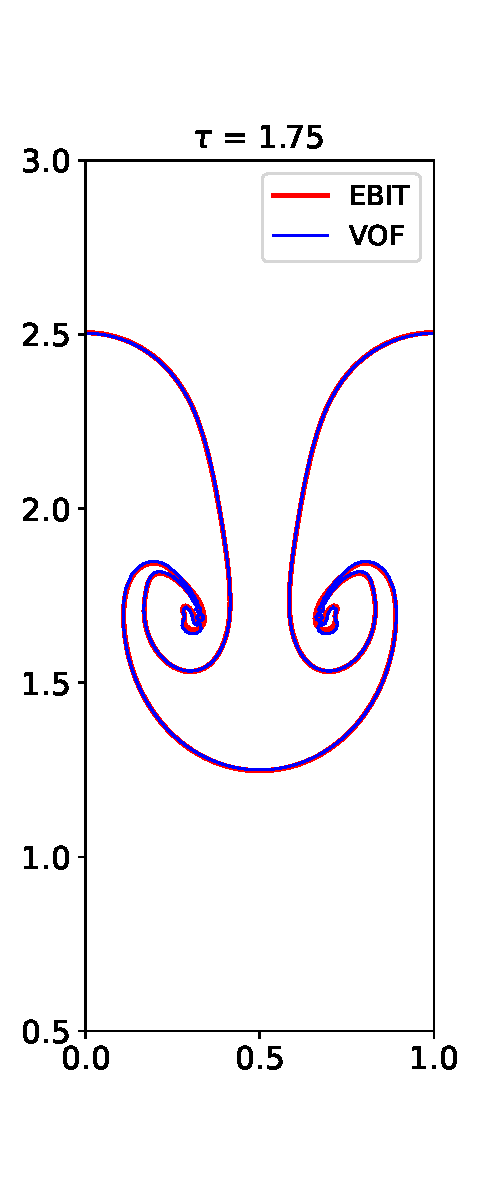
\includegraphics[width=0.25\textwidth]{rti_intf_3} \\
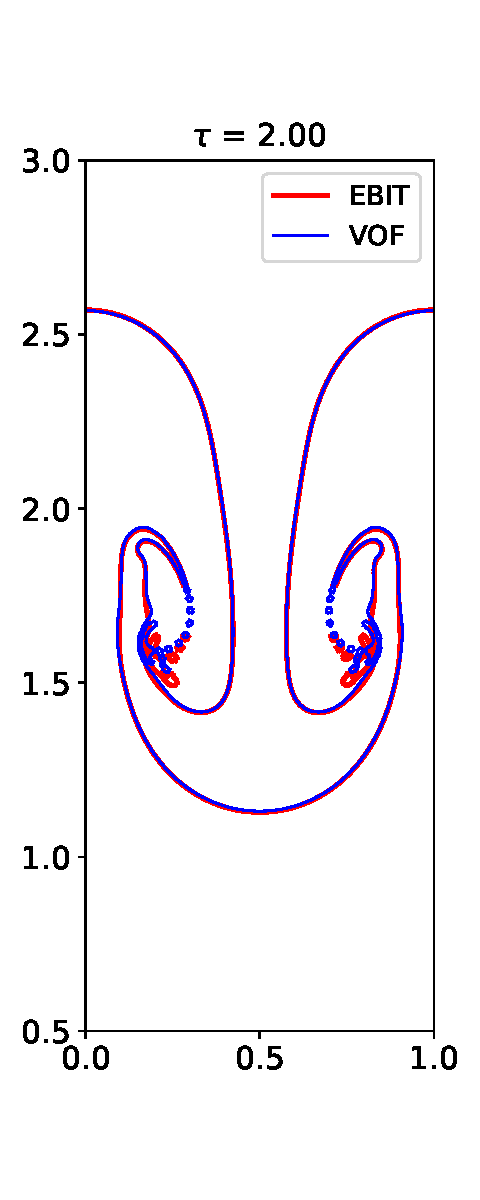
\includegraphics[width=0.25\textwidth]{rti_intf_4} &
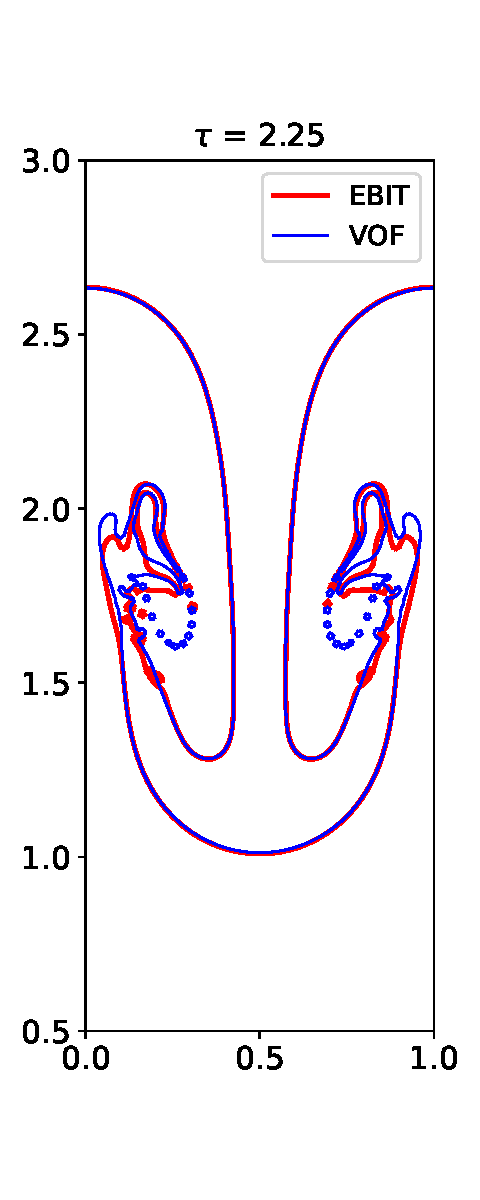
\includegraphics[width=0.25\textwidth]{rti_intf_5} &
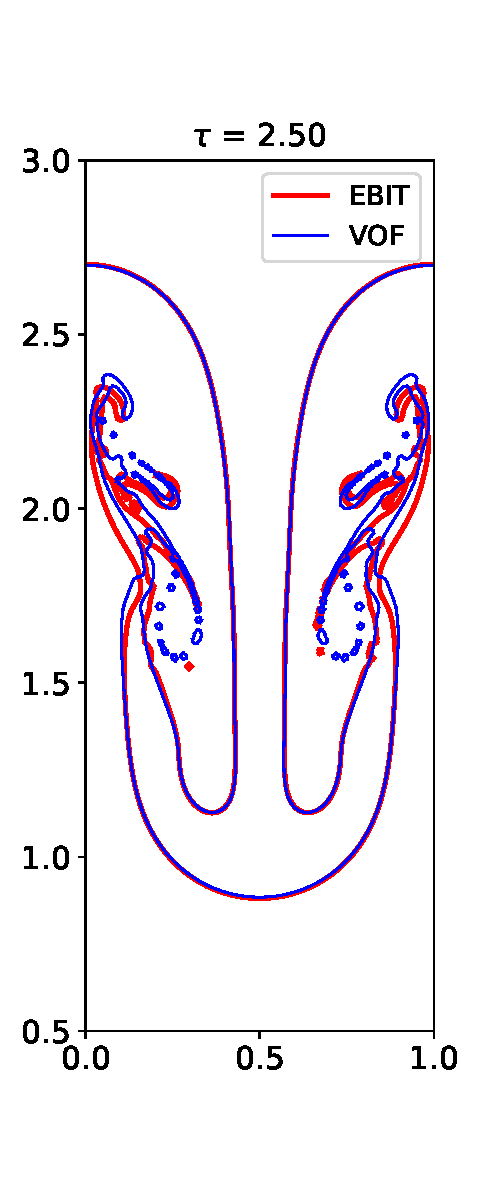
\includegraphics[width=0.25\textwidth]{rti_intf_6} 
\end{tabular}
\end{center}
\caption{Rayleigh-Taylor instability test with different methods: interface lines at dimensionless times $\tau = 1.,1.5,1.75,2.,2.25,2.5$.}
\label{Fig_rti_intfs}
\end{figure}
% ----------
\begin{figure}
\centering
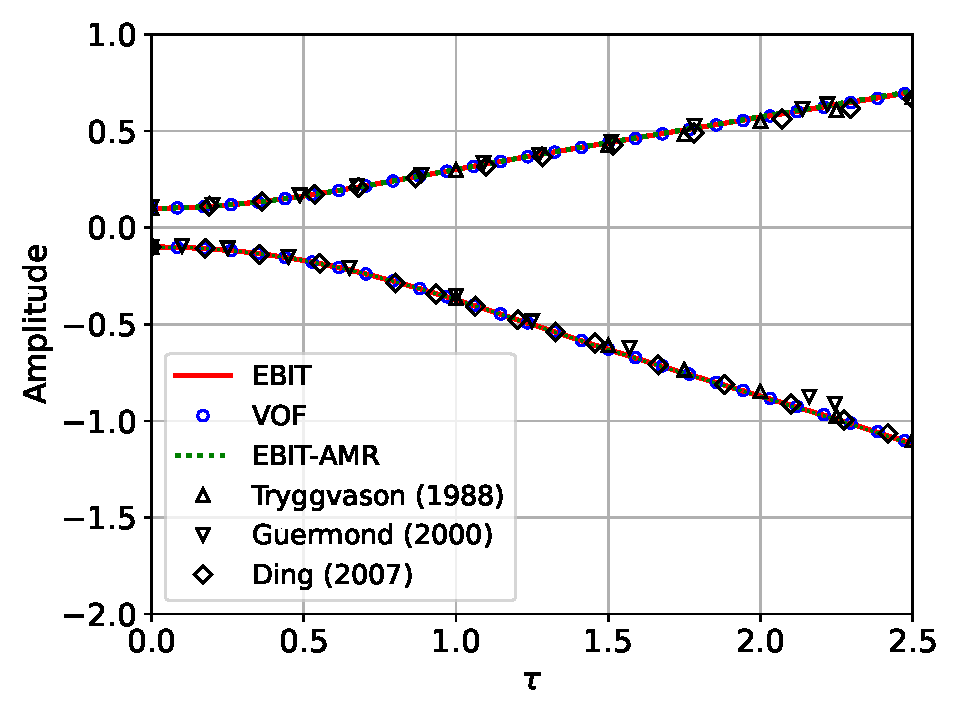
\includegraphics[width=\textwidth]{rti_amp}
\caption{Rayleigh-Taylor instability test with different methods: highest and lowest positions of the interface, with respect to the mean position at $y=2$, as a function 
of dimensionless time $\tau$.}
\label{Fig_rti_amp}
\end{figure}
% ----------

The results of the simulation are first presented in Fig.~\ref{Fig_rti_intfs} with the representation of the interface line at several dimensionless times 
$\tau = t \sqrt{g\, At / d}$. Overall, these results compare rather well with those presented in \cite{Ding_2007_226}.

More specifically, in the early stages of the simulation, $\tau \leq 1.75$, the shape of interface calculated with the new EBIT method and that with the PLIC-VOF method are in very good agreement, small discrepancies are observed only in the roll-up region where complex structures with thin ligaments start to develop. 

Some remarkable differences occur at later times ($\tau \geq 2.00$) when the ligaments start to break up. Due to the mass conservation property of the PLIC-VOF method, many small droplets are formed when the ligaments tear apart. However, in the new EBIT method, these small droplets will soon disappear due to the topology change mechanism. Thus, in the roll-up region, the interface structure obtained with the new EBIT method agrees only qualitatively with that of the PLIC-VOF method.

In spite of this local but consistent difference, very good agreement is observed for the highest and lowest positions of the interface during the whole simulation. The highest
position of the rising fluid, near the two vertical boundaries at $x=0$ and $x=d$,
and the lowest position of the falling fluid, near the centerline at $x=d/2$, both computed
with respect to the mean position at $y = 2\,d$, are shown in Fig.~\ref{Fig_rti_amp}. They are in very good agreement with the results obtained with the PLIC-VOF method and those by Tryggvason \cite{Tryggvason_1988_75}, Guermond \cite{ Guermond_2000_165} and Ding \cite{Ding_2007_226}.

% ----------
\begin{figure}
\begin{center}
\begin{tabular}{ccc}
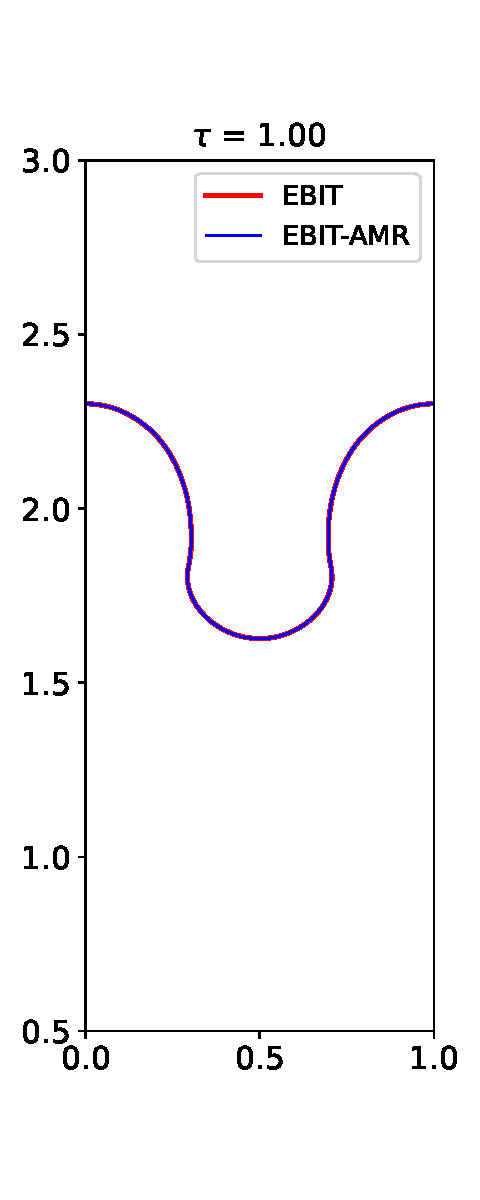
\includegraphics[width=0.22\textwidth]{rti_intf_amr_1} &
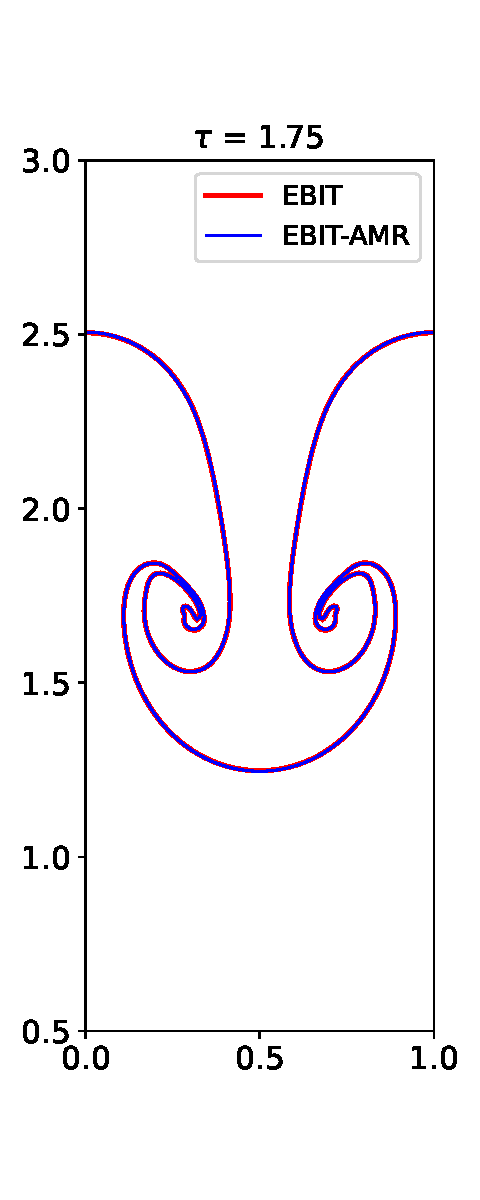
\includegraphics[width=0.22\textwidth]{rti_intf_amr_2} &
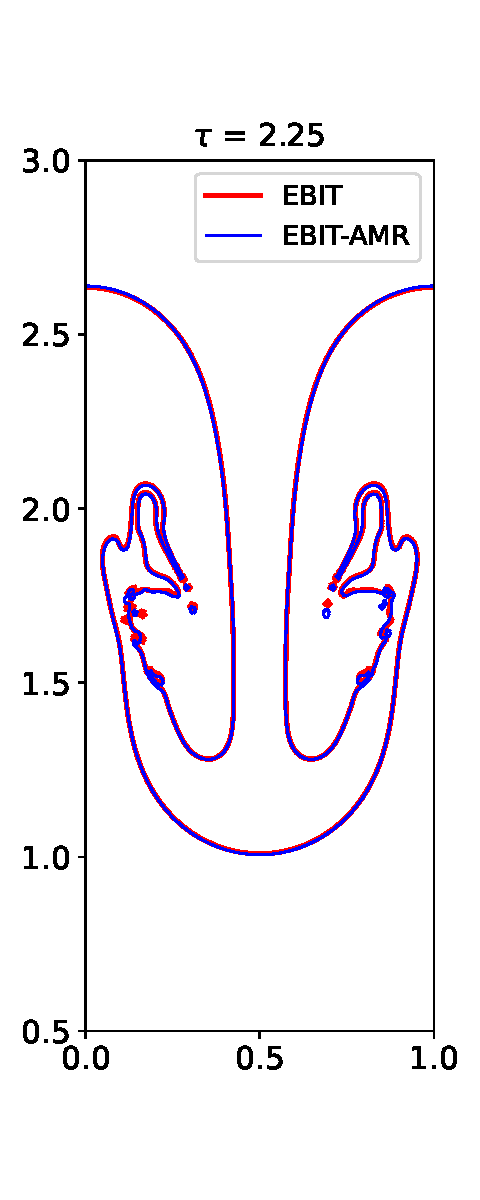
\includegraphics[width=0.22\textwidth]{rti_intf_amr_3} \\
 & (a) & \\[2pt]          
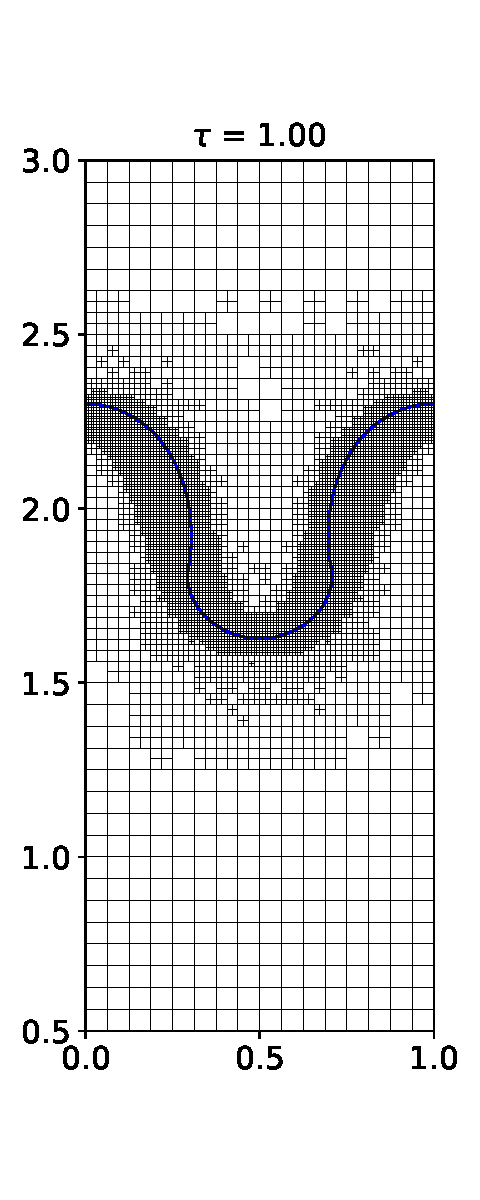
\includegraphics[width=0.22\textwidth]{rti_grid_amr_1} &
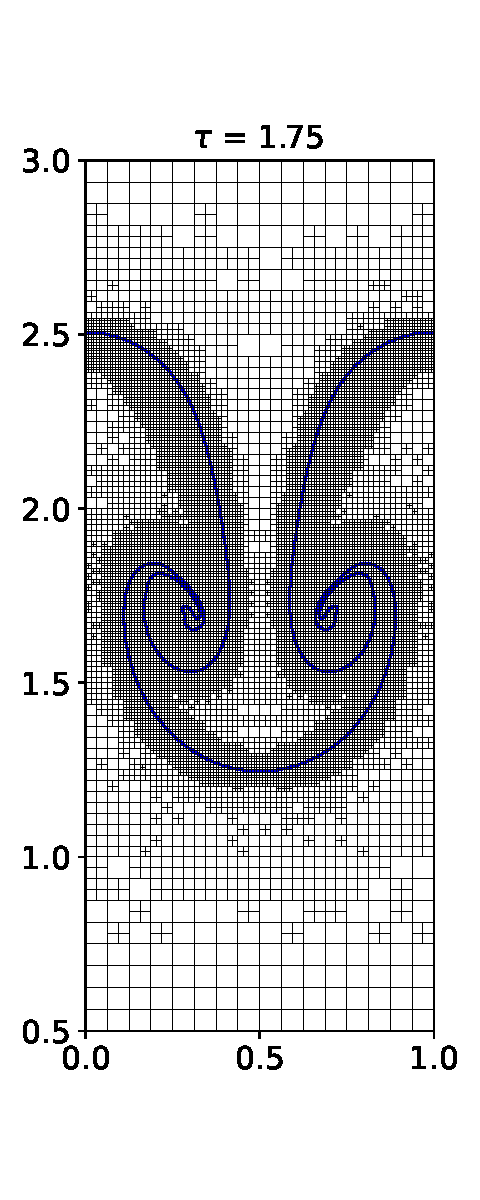
\includegraphics[width=0.22\textwidth]{rti_grid_amr_2} &
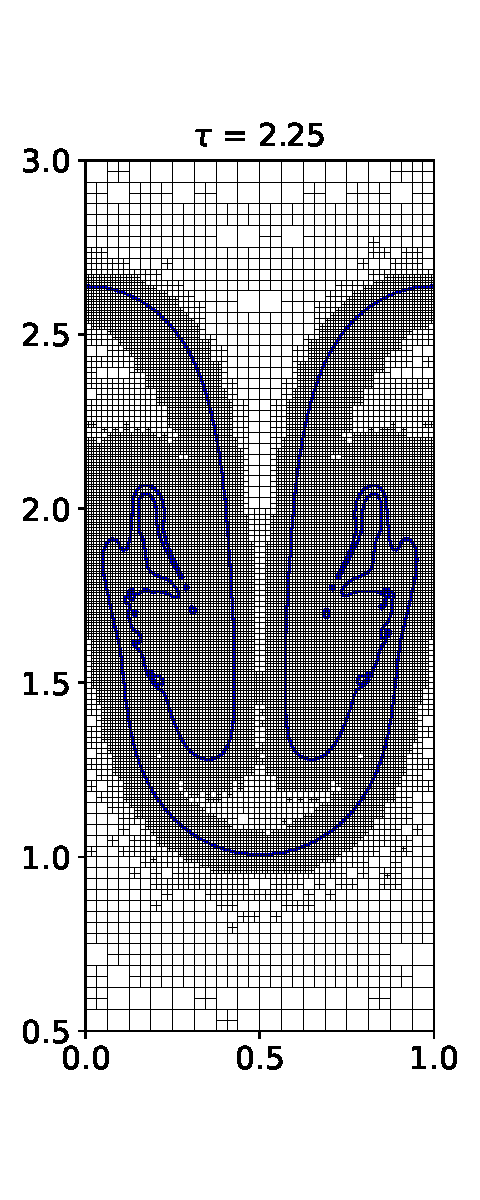
\includegraphics[width=0.22\textwidth]{rti_grid_amr_3} \\
 & (b) & 
\end{tabular}
\end{center}
\caption{Rayleigh-Taylor instability test at dimensionless times $\tau = 1.,1.75,2.25$: (a) interface lines with and without AMR; (b) computational grid with $N_{l,max}=9$ and $N_{l,min}=6$.}
\label{Fig_rti_intfs_amr}
\end{figure}
% ----------

% ----------
\begin{table}[hbt!]
\caption{Computational efficiency of the EBIT method with AMR, Rayleigh-Taylor instability test, $N_{l,max}=9$ and $N_{l,min}=6$.}
\centering
\begin{tabular}{cccc}
\hline 
 Method & Number of (leaf) cells & Time steps & Wall time (s) \\ 
\hline 
EBIT & $65536$ & $5656$ & $1741$ \\ 
EBIT-AMR & $27355$ & $5656$ & $207$ \\ 
\hline
VOF & $65536$ & $5656$ & $914$ \\ 
VOF-AMR & $27223$ & $5656$ & $151$ \\ 
\hline 
\end{tabular}
\label{Tab_rti_amr}
\end{table}
% ----------

The interface lines obtained with the new EBIT method combined with AMR are finally shown in Fig.~\ref{Fig_rti_intfs_amr}. The maximum level of refinement is now $N_{l,max}=9$, while the minimum level is $N_{l,min}=6$. The refinement criteria are based not only on the position of the interface, but also on the velocity gradient, thus the cells within the roll-up region, characterized by a strong vorticity, are also refined to the maximum level, even if they are not very close to the interface (see Fig.~\ref{Fig_rti_intfs_amr}b). The interface lines calculated with the new EBIT method on the quadtree grid agree rather well with those on the fixed Cartesian grid (see Fig.~\ref{Fig_rti_intfs_amr}a), only minor differences are observed in the roll-up region.

The computational efficiency for this test of the new EBIT method with or without AMR is summarized in Table~\ref{Tab_rti_amr}. The wall time shown in the table includes both the interface advection and the Navier--Stokes solver. For the PLIC-VOF method with AMR (VOF-AMR), the mesh refinement criteria are based on both curvature and velocity gradient. Without AMR, the dynamics with the new EBIT method is about 2 times slower than with the PLIC-VOF method. 
When AMR is used, the wall times for the two methods are comparable. But the EBIT method still presents an about $33\%$ increase in the wall time. The lower efficiency of the EBIT method can be due to several reasons: i) The PLIC-VOF method updates the volume fractions directly. But for the EBIT method, both the position of markers and the value of Color Vertex need to be updated to calculate the volume fractions. Thus, more computation is involved in each advection step. ii) Since the connectivity of marker is represented by the Color Vertex implicitly, we need to access both the position of markers and the Color Vertex when we update each related field. Consequently, more memory access is involved in the advection step, which slows down the algorithm. iii) The PLIC-VOF method in Basilisk exists for more than decade and its efficiency has been highly optimized. In this work, we focus more on the accuracy of the EBIT method instead of its efficiency. Definitely, further improvement of the computational efficiency of the EBIT method is one of our goals.

For the simulation on a Cartesian grid, the area error is $E_{area} = 3.50 \times 10^{-3}$, which is much larger than that measured in the capillary wave test, $E_{area} = 5.3 \times 10^{-6}$. Here, topology changes take place at the later stages of the simulation and small droplets will be removed by the topology change mechanism.

\subsection{Rising bubble}

In this test we examine a single bubble rising under buoyancy inside a heavier fluid. This test case was first proposed by Hysing \cite{Hysing_2009_60} and it provides a standard benchmark for multiphase flow simulations, since this configuration is simple enough to be simulated accurately. Nevertheless, the bubble shows a strong deformation and even complex topology changes in some flow regimes \cite{Clift_1978, Legendre_2022_07}, thus giving an adequate challenge to interface tracking techniques. 

By taking into account the symmetry with respect to the vertical axis, we consider the rectangular computational domain $[0, D] \times [0, 4\,D]$, with $D=0.5$, partitioned with $N_x \times N_y = 128 \times 512$ grid cells. At the beginning of the simulation, a circular bubble of radius $R=D/2$ is positioned in the bottom part of the domain with center at $(0, D)$.
A no-slip boundary condition is enforced at the bottom and at the top of the computational domain, a free-slip boundary condition on the right vertical wall and a symmetric boundary condition on the left vertical boundary. The value of the relevant physical properties is that provided by Hysing \cite{Hysing_2009_60} and is listed in Table~\ref{Tab_para_rising},
where $Re = \big( \rho_1 g^{1/2} d^{3/2} \big) \big/ \mu_1$ is the Reynolds number and
$Bo = \big( \rho_1 g L^2 \big) \big/ \sigma$ the Bond number. In the following simulations, the timestep is limited by both the $CFL$ number, $CFL=0.5$, and the period of the shortest capillary, see Eq.~\eqref{Eq_dt_cap}.

% ----------
\begin{table}[hbt!]
\caption{Physical properties for the rising bubble test.}
\centering
\begin{tabular}{ccccccccc}
\hline 
 Test case &$\rho_1$& $\rho_2$& $\mu_1$ & $\mu_2$ & $g$ & $\sigma$ & $Re$ & $Bo$ \\ 
\hline 
$1$ &$1000 $ & $100$ & $ 10$ & $1$ & $0.98$ &$24.5$ & $35$ & $10$ \\ 
$2$ &$1000 $ & $1$ & $ 10$ & $0.1$ & $0.98$ &$1.96$ & $35$ & $125$ \\ 
\hline 
\end{tabular}
\label{Tab_para_rising}
\end{table}
% ----------
We consider the two different test cases of Table~\ref{Tab_para_rising}. In the first test, the bubble should end up in the ellipsoidal regime \cite{Hysing_2009_60}, since the surface tension forces are strong enough to hold the bubble together, hence no breakup is present in the simulation. For this first case, we solve both the axisymmetric problem and the two-dimensional Cartesian one.

The interface lines at the end of the simulation at time $t = 3$ are shown in Fig.~\ref{Fig_rising_intfs}a, for both the axisymmetric and Cartesian problems and with the new EBIT and PLIC-VOF methods. In general, good agreement is found between the two methods in both problems. More particularly, the bubble computed with the PLIC-VOF method
is always a very little ahead of the bubble with the new EBIT method.

The rising velocities for the two problems and the two methods as a function of time are shown in Fig.~\ref{Fig_rising_vel}a. The figure includes also the results obtained with the new EBIT method in conjunction with AMR. The profiles of the rising velocities are very close to each other and this justify the fact that at the end of the simulation there is very little difference between the interface lines. For the Cartesian problem, the value of the maximum rising velocity is $0.2419$ for the new EBIT method and $0.2418$ for the PLIC-VOF method, which are basically the same value, $0.2419 \pm 0.0002$, reported by Hysing \cite{Hysing_2009_60}.


In the second test, the bubble lies somewhere between the skirted and the dimpled ellipsoidal-cap regimes, indicating that breakup can eventually take place. The simulation is carried out with both the new EBIT and PLIC-VOF methods, and the interface lines at the end of the simulation at time $t = 3$ are shown in Fig.~\ref{Fig_rising_intfs}b. At the given mesh resolution, the bubble skirt is observed with both methods, with no interface breakup.
Good agreement is observed between the two interface lines. More in detail, the new EBIT method predicts a slightly larger central part of the bubble and a smoother and shorter tail in the skirt region.

The rising velocities for the two methods as a function of time are shown in Fig.~\ref{Fig_rising_vel}b. In this case as well, the figure includes the results
obtained with the new EBIT method in conjunction with AMR. The presence of two peaks is well predicted in our simulation. The value of the first one is $0.2507$ for the new EBIT method and $0.2512$ for the PLIC-VOF method, in good agreement with the value $0.25 \pm 0.01$
indicated by Hysing \cite{Hysing_2009_60}.

% ----------
\begin{figure}
\begin{center}
\begin{tabular}{cc}
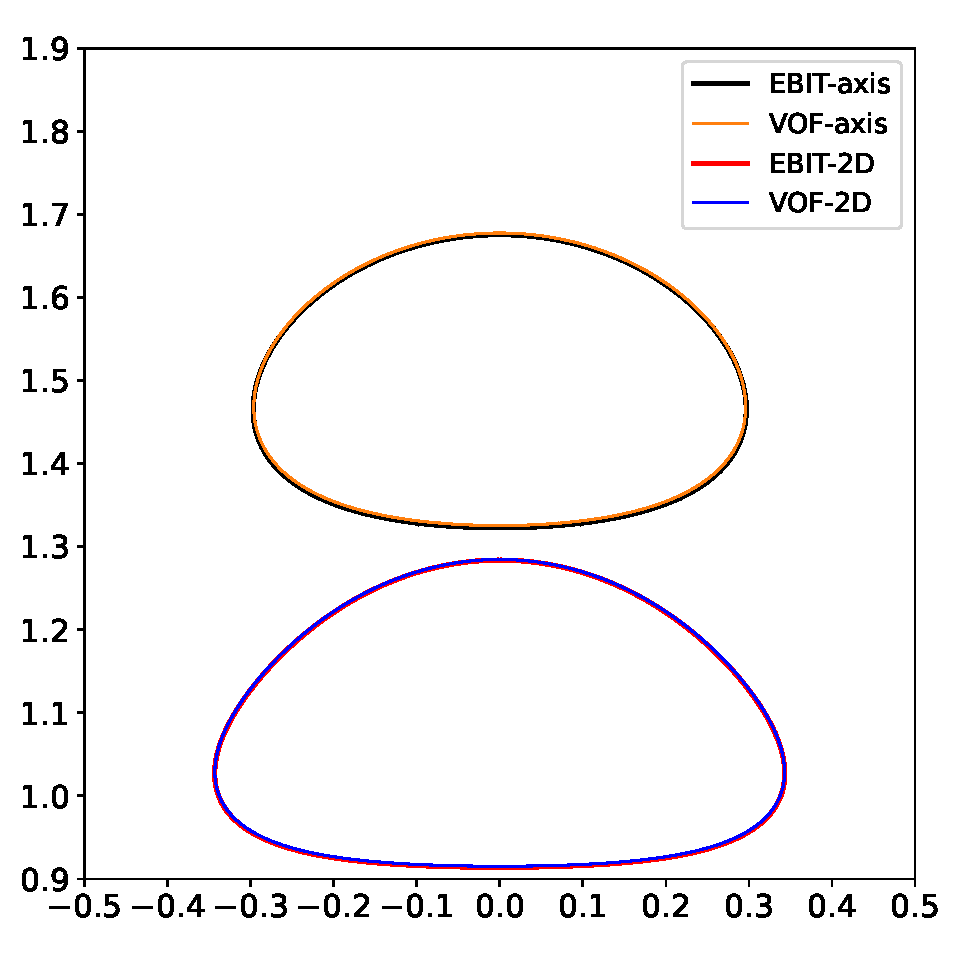
\includegraphics[width=0.45\textwidth]{shape_c1} &
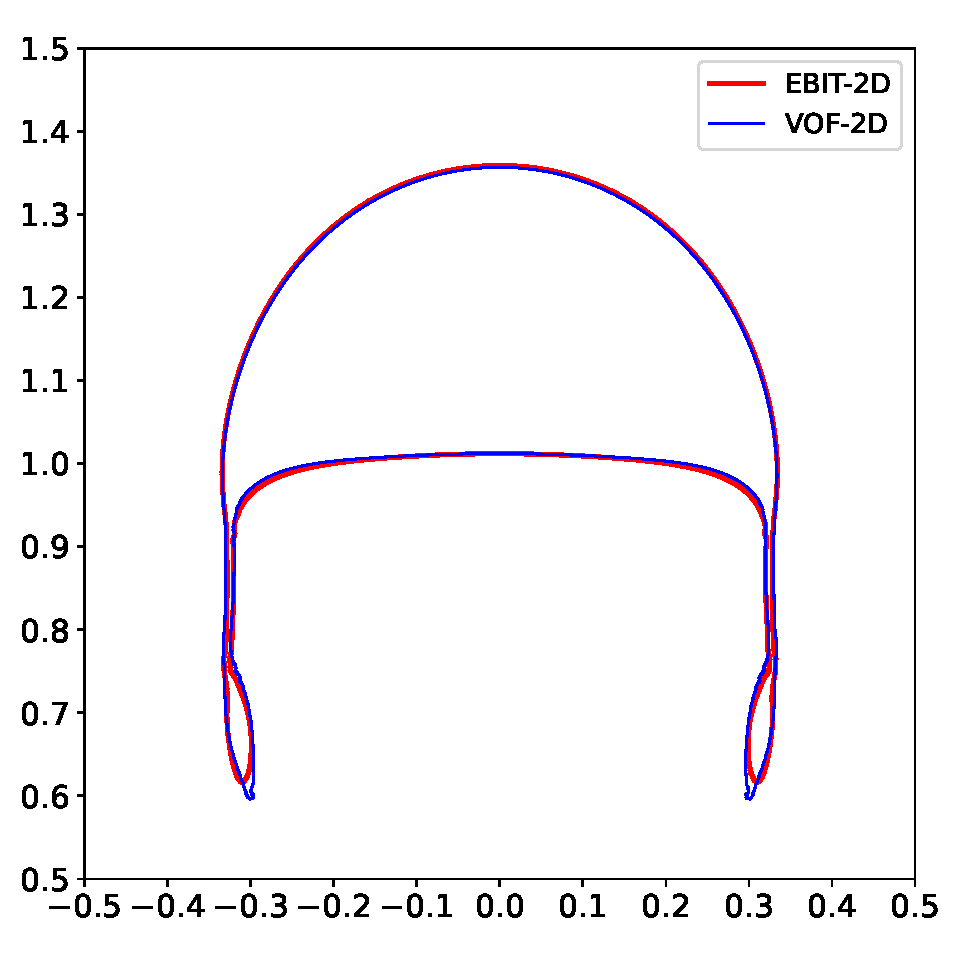
\includegraphics[width=0.45\textwidth]{shape_c2}\\
(a) & (b) 
\end{tabular}
\end{center}
\caption{Rising bubble test. Interface lines at the end of the simulation $t = 3$ with different methods: (a) axisymmetric and Cartesian solutions for test case 1; (b) Cartesian solution for test case 2.}
\label{Fig_rising_intfs}
\end{figure}
% ----------

% ----------
% rising velocity
\begin{figure}
\begin{center}
\begin{tabular}{cc}
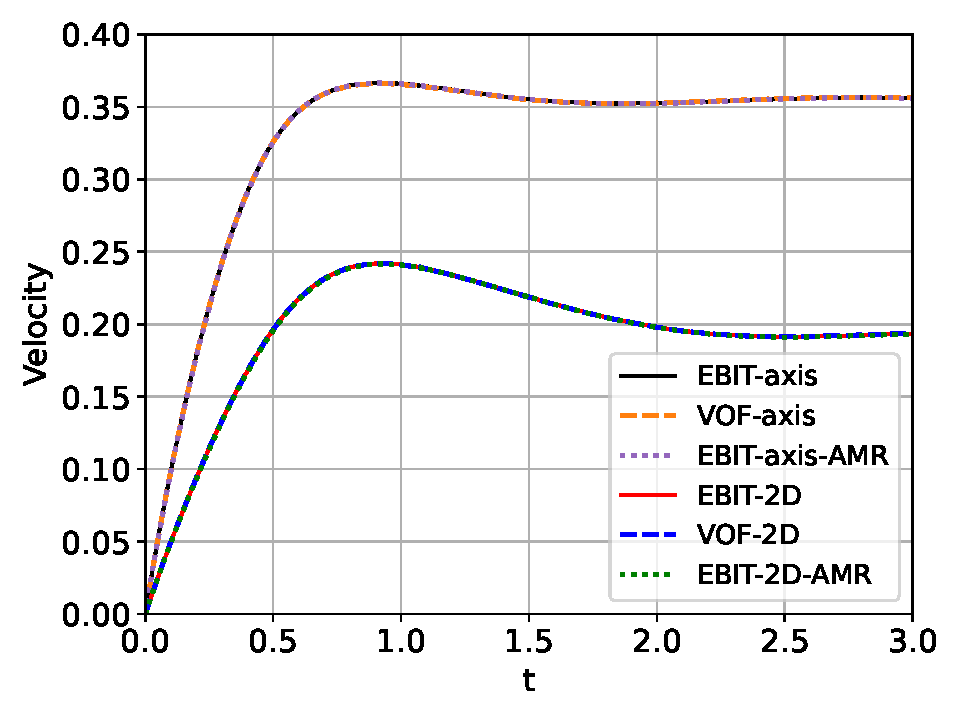
\includegraphics[width=0.45\textwidth]{vel_c1} &
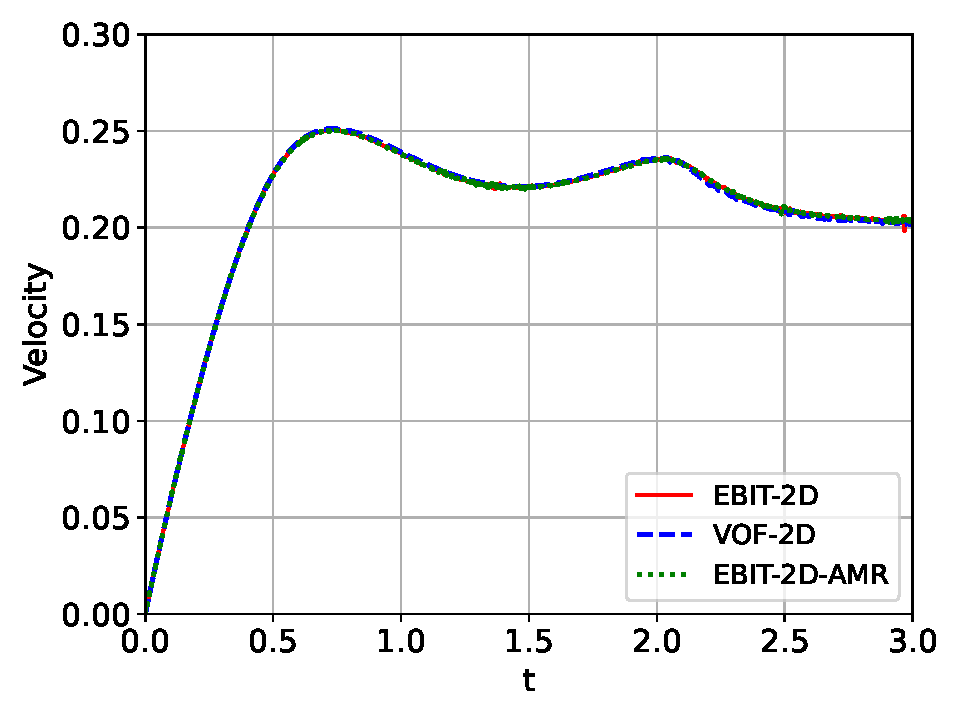
\includegraphics[width=0.45\textwidth]{vel_c2}\\
(a) & (b) 
\end{tabular}
\end{center}
\caption{Rising bubble test. Bubble velocities as a function of time with different methods: (a) profiles for test case 1, including EBIT with AMR; (b) profiles for test case 2, including EBIT with AMR.}
\label{Fig_rising_vel}
\end{figure}
% ----------


% ----------
\begin{figure}
\begin{center}
\begin{tabular}{cc}
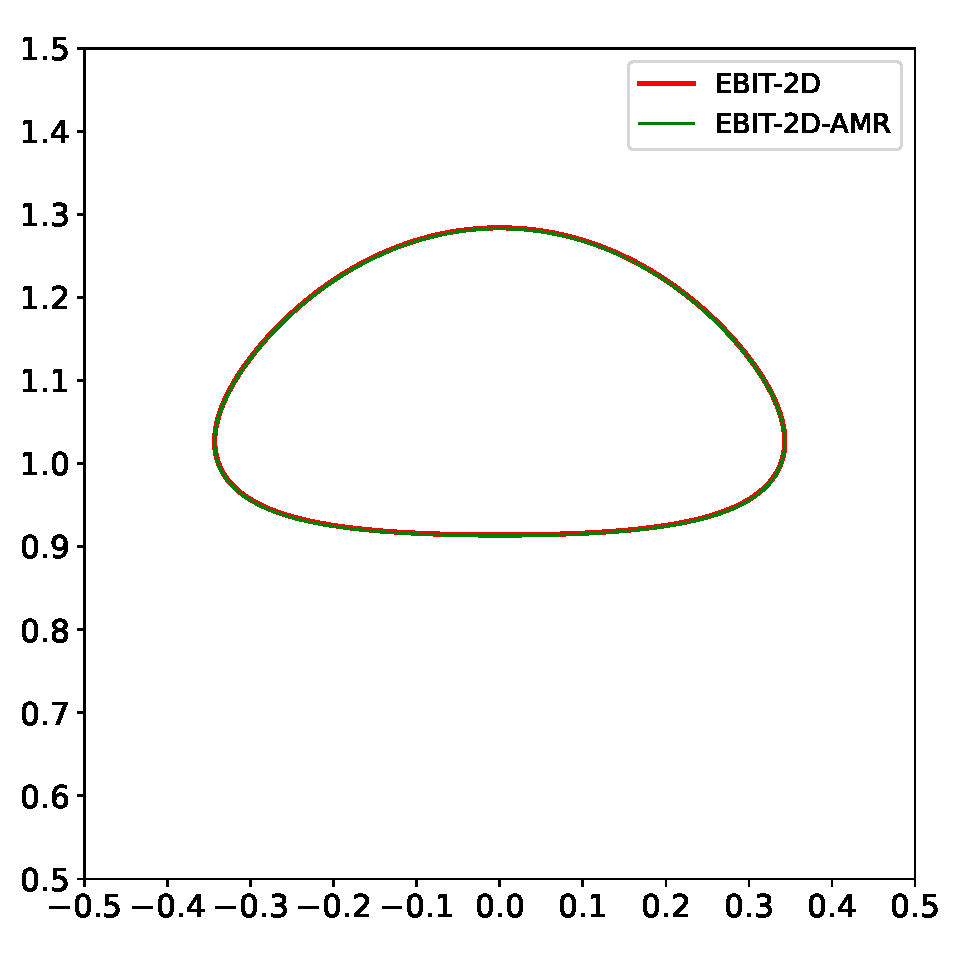
\includegraphics[width=0.45\textwidth]{shape_c1_amr_1} &
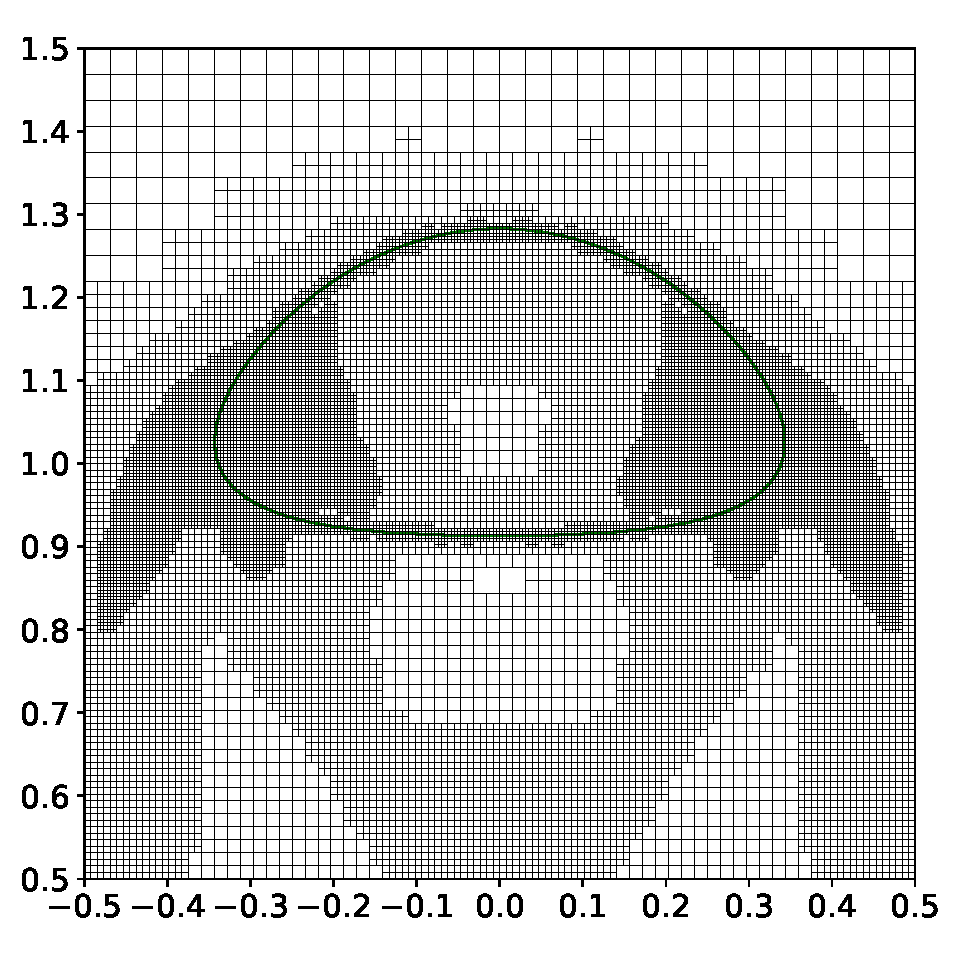
\includegraphics[width=0.45\textwidth]{shape_c1_amr_2}\\
(a) & (b) 
\end{tabular}
\end{center}
\caption{Rising bubble test case 1-2D: (a) interface lines at the end of the simulation $t = 3$ with and without AMR; (b) computational grid with $N_{l,max}=9$ and $N_{l,min}=6$.}
\label{Fig_rising_intfs_c1_amr}
\end{figure}
% ----------


% ----------
\begin{figure}
\begin{center}
\begin{tabular}{cc}
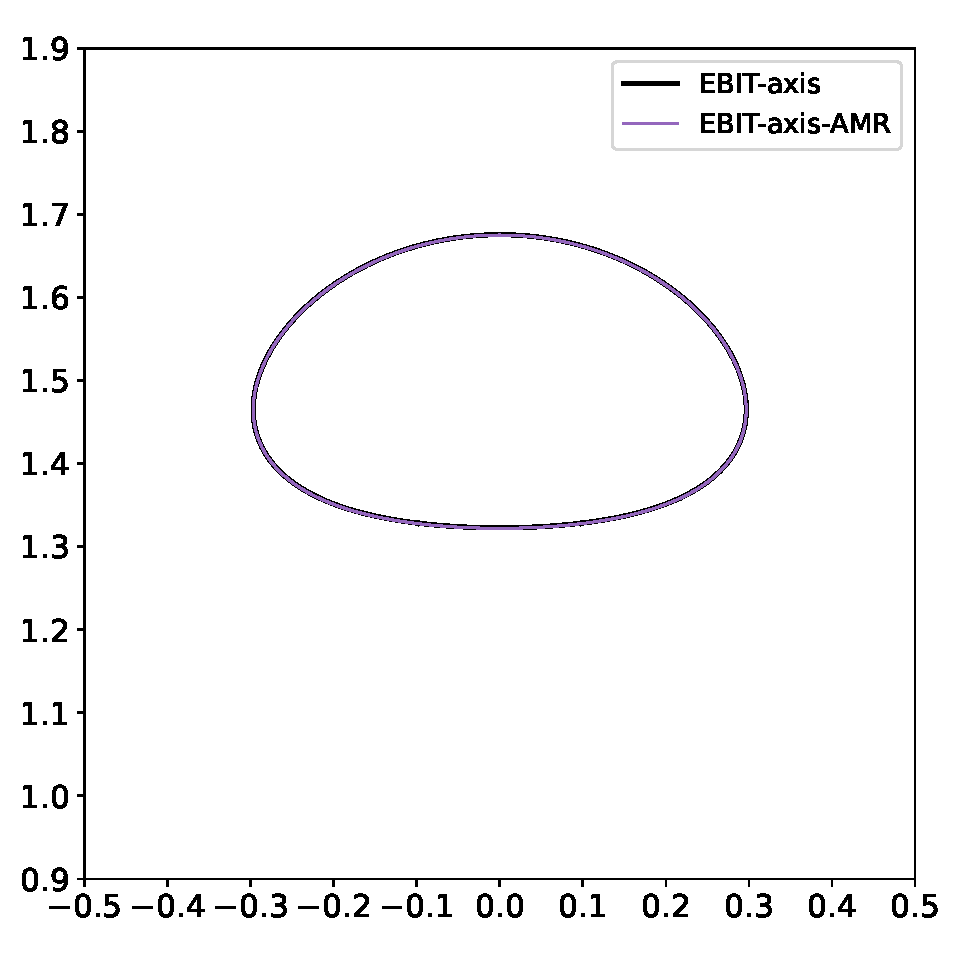
\includegraphics[width=0.45\textwidth]{shape_c1_axi_amr_1} &
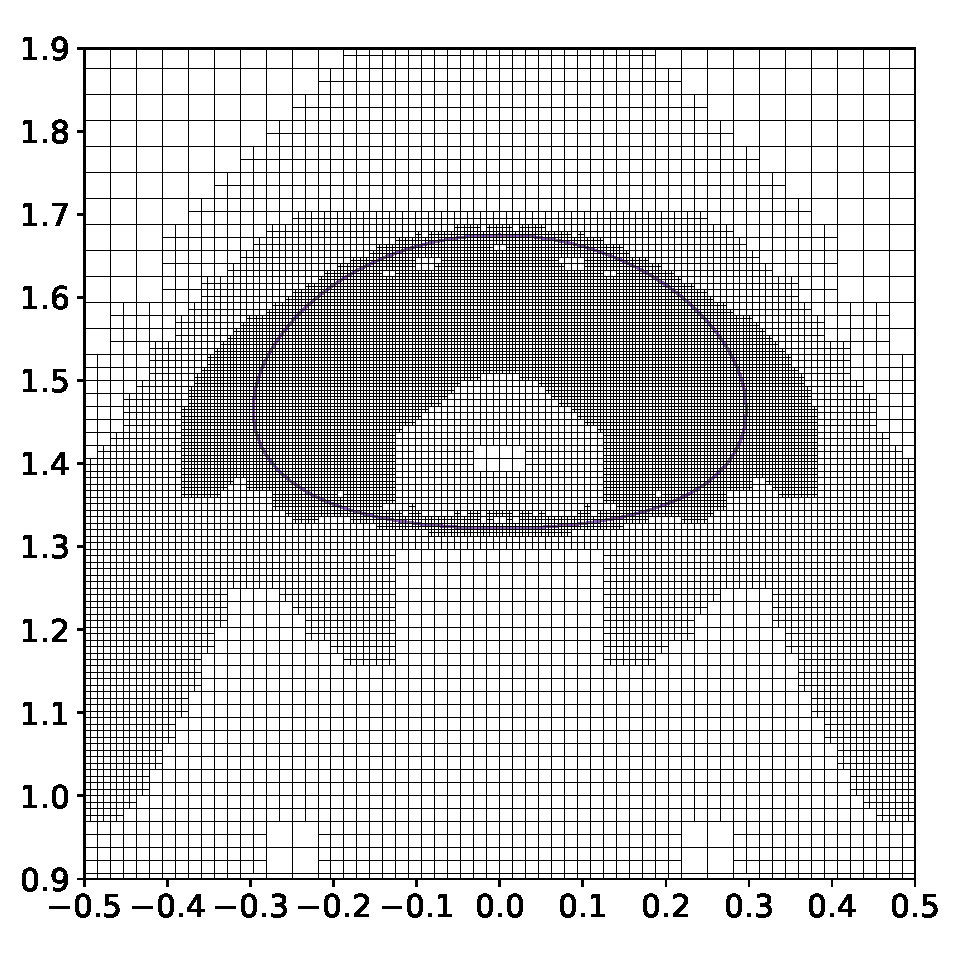
\includegraphics[width=0.45\textwidth]{shape_c1_axi_amr_2}\\
(a) & (b) 
\end{tabular}
\end{center}
\caption{Rising bubble test case 1-Axisymmetric: (a) interface lines at the end of the simulation $t = 3$ with and without AMR; (b) computational grid with $N_{l,max}=9$ and $N_{l,min}=6$.}
\label{Fig_rising_intfs_c1_axi_amr}
\end{figure}
% ----------

% ----------
\begin{figure}
\begin{center}
\begin{tabular}{cc}
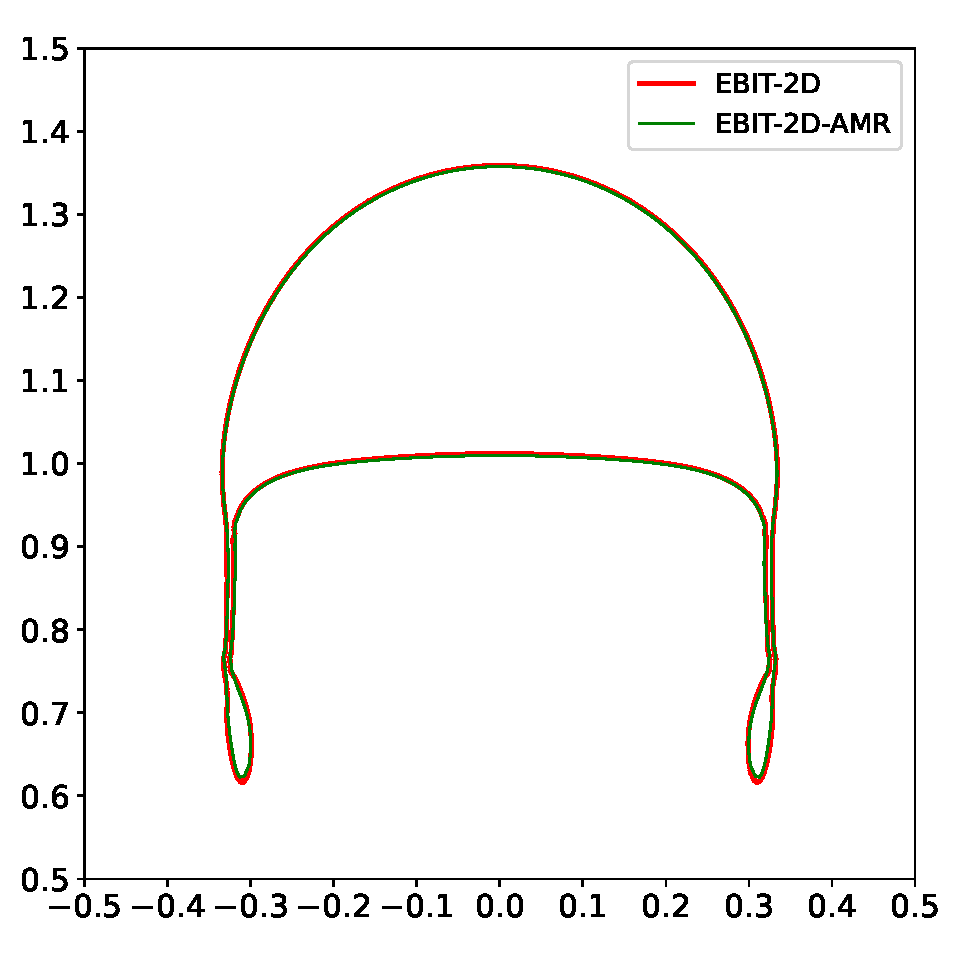
\includegraphics[width=0.45\textwidth]{shape_c2_amr_1} &
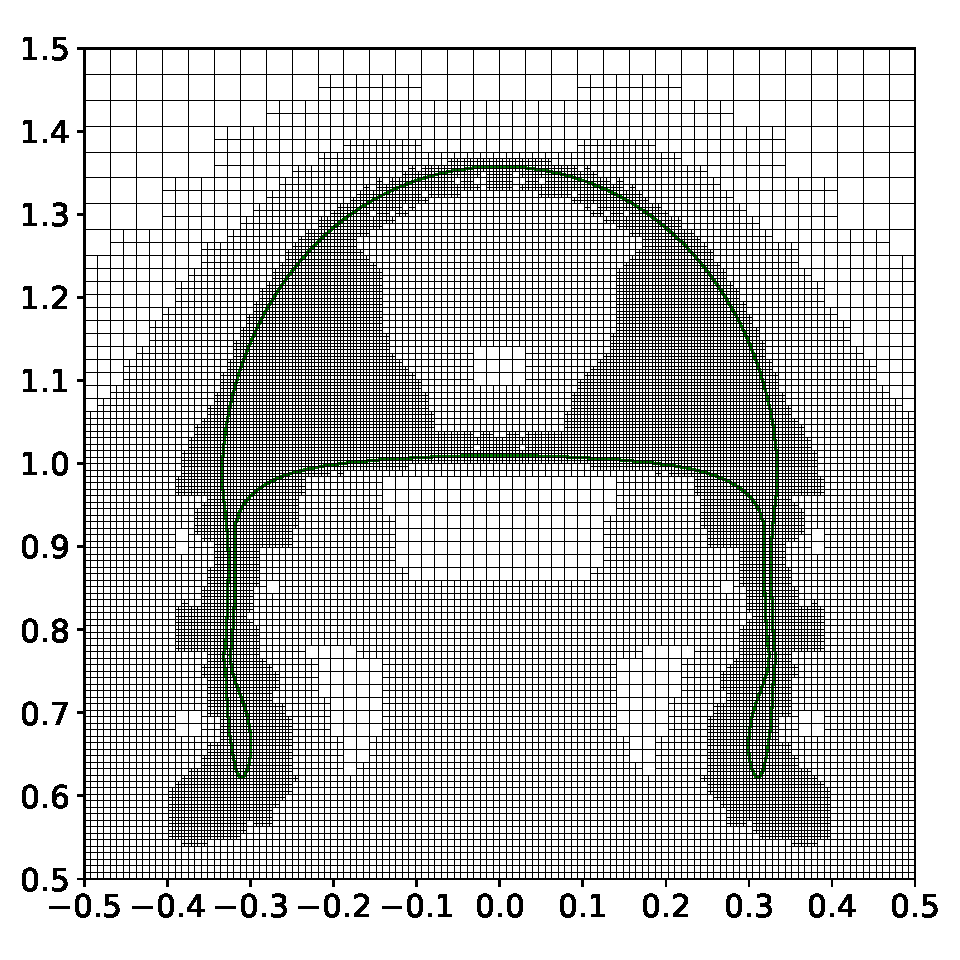
\includegraphics[width=0.45\textwidth]{shape_c2_amr_2}\\
(a) & (b) 
\end{tabular}
\end{center}
\caption{Rising bubble test case 2-2D: (a) interface lines at the end of the simulation $t = 3$ with and without AMR; (b) computational grid with $N_{l,max}=9$ and $N_{l,min}=6$.}
\label{Fig_rising_intfs_c2_amr}
\end{figure}
% ----------

% ----------
\begin{table}[hbt!]
\caption{Computational efficiency of the EBIT method with AMR, rising bubble test, $N_{l,max}=9$ and $N_{l,min}=6$.}
\centering
\begin{tabular}{ccccc}
\hline 
 &Method & Number of (leaf) cells & Time steps & Wall time (s) \\ 
\hline 
Case1-2D& EBIT & $65536$ & $4606$ & $1726$ \\ 
&EBIT-AMR & $11077$ & $4606$ & $172$ \\ 
&VOF & $65536$ & $4607$ & $935$ \\ 
&VOF-AMR & $10852$ & $4607$ & $147$ \\ 
\hline 
Case1-Axi & EBIT & $65536$ & $4606$ & $1824$ \\ 
&EBIT-AMR & $10141$ & $4606$ & $166$ \\ 
&VOF & $65536$ & $4607$ & $1136$ \\ 
&VOF-AMR & $9937$ & $4607$ & $145$ \\ 
\hline 
Case2-2D& EBIT & $65536$ & $1599$ & $4653$ \\ 
&EBIT-AMR & $14392$ & $1595$ & $729$ \\ 
&VOF & $65536$ & $1636$ & $2822$ \\ 
&VOF-AMR & $14095$ & $1634$ & $610$ \\ 
\hline 
\end{tabular}
\label{Tab_rising_amr}
\end{table}
% ----------

When AMR is considered, the refinement criteria are those that have been used in the Rayleigh-Taylor instability test, i.e. proximity to the interface and velocity gradient. 
The maximum level of refinement is $N_{l,max}=9$, while the minimum level is $N_{l,min}=6$, for both test cases.
The interface lines at the end of the simulation at time $t = 3$ are shown in Figs.~\ref{Fig_rising_intfs_c1_amr} and \ref{Fig_rising_intfs_c1_axi_amr} for test case 1, and
in Fig.~\ref{Fig_rising_intfs_c2_amr} for test case 2.

For the axisymmetric problem, the interface line calculated by the new EBIT method on the quadtree grid is on top of the line on the fixed Cartesian grid. For the two Cartesian problems, the interface line on the quadtree grid is just a little bit behind that on the fixed Cartesian grid.

The computational efficiency for these two cases of the new EBIT method with
or without AMR is summarized in Table~\ref{Tab_rising_amr}. Without AMR, the new EBIT method represents a $60\%$ to $85\%$ increase in wall time compared to the PLIC-VOF method, which is smaller than that shown in the Rayleigh-Taylor instability test. When AMR is used, this increase becomes less than $20\%$ for all cases.

For the simulations on a Cartesian grid, the area errors $E_{area}$ for case1-2D, case1-Axi and case2-2D are $1.11 \times 10^{-4}$, $2.00 \times 10^{-4}$ and $4.56 \times 10^{-4}$, respectively, which are one order of magnitude smaller than those in the Rayleigh-Taylor instability test with topology changes. Furthermore, the case2-2D with a thin skirt structure shows a larger area loss.